	\documentclass[10pt,a4paper]{article}
\usepackage[utf8]{inputenc}
\usepackage[spanish]{babel}
\usepackage{amsmath}
\usepackage{amsfonts}
\usepackage{amssymb}
\usepackage{graphicx}
\usepackage{float}
	\usepackage[left=2cm,right=2cm,top=2cm,bottom=2cm]{geometry}
\usepackage{circuitikz}
\usepackage{tikz}
\usepackage{tikz-timing}
\usetikztiminglibrary[rising arrows]{clockarrows}
\usepackage{pgfplots}
\pgfplotsset{compat=1.15}
\usetikzlibrary{matrix,calc}
\usepackage{listings}

\usepackage[export]{adjustbox}
\usepackage{graphicx,wrapfig,lipsum}
\usepackage{booktabs}
\usepackage[skip=0pt]{caption}
\captionsetup[figure]{font=small,labelfont=small}

\usepackage{pdfpages}
\usepackage{lscape}
\usepackage{multicol}
\usepackage{multirow}
\usepackage{wrapfig}


\usetikzlibrary{matrix,calc}

%isolated term
%#1 - Optional. Space between node and grouping line. Default=0
%#2 - node
%#3 - filling color
\newcommand{\implicantsol}[3][0]{
    \draw[rounded corners=3pt, fill=#3, opacity=0.3] ($(#2.north west)+(135:#1)$) rectangle ($(#2.south east)+(-45:#1)$);
    }


%internal group
%#1 - Optional. Space between node and grouping line. Default=0
%#2 - top left node
%#3 - bottom right node
%#4 - filling color
\newcommand{\implicant}[4][0]{
    \draw[rounded corners=3pt, fill=#4, opacity=0.3] ($(#2.north west)+(135:#1)$) rectangle ($(#3.south east)+(-45:#1)$);
    }

%group lateral borders
%#1 - Optional. Space between node and grouping line. Default=0
%#2 - top left node
%#3 - bottom right node
%#4 - filling color
\newcommand{\implicantcostats}[4][0]{
    \draw[rounded corners=3pt, fill=#4, opacity=0.3] ($(rf.east |- #2.north)+(90:#1)$)-| ($(#2.east)+(0:#1)$) |- ($(rf.east |- #3.south)+(-90:#1)$);
    \draw[rounded corners=3pt, fill=#4, opacity=0.3] ($(cf.west |- #2.north)+(90:#1)$) -| ($(#3.west)+(180:#1)$) |- ($(cf.west |- #3.south)+(-90:#1)$);
}

%group top-bottom borders
%#1 - Optional. Space between node and grouping line. Default=0
%#2 - top left node
%#3 - bottom right node
%#4 - filling color
\newcommand{\implicantdaltbaix}[4][0]{
    \draw[rounded corners=3pt, fill=#4, opacity=0.3] ($(cf.south -| #2.west)+(180:#1)$) |- ($(#2.south)+(-90:#1)$) -| ($(cf.south -| #3.east)+(0:#1)$);
    \draw[rounded corners=3pt, fill=#4, opacity=0.3] ($(rf.north -| #2.west)+(180:#1)$) |- ($(#3.north)+(90:#1)$) -| ($(rf.north -| #3.east)+(0:#1)$);
}

%group corners
%#1 - Optional. Space between node and grouping line. Default=0
%#2 - filling color
\newcommand{\implicantcantons}[2][0]{
    \draw[rounded corners=3pt, opacity=.3] ($(rf.east |- 0.south)+(-90:#1)$) -| ($(0.east |- cf.south)+(0:#1)$);
    \draw[rounded corners=3pt, opacity=.3] ($(rf.east |- 8.north)+(90:#1)$) -| ($(8.east |- rf.north)+(0:#1)$);
    \draw[rounded corners=3pt, opacity=.3] ($(cf.west |- 2.south)+(-90:#1)$) -| ($(2.west |- cf.south)+(180:#1)$);
    \draw[rounded corners=3pt, opacity=.3] ($(cf.west |- 10.north)+(90:#1)$) -| ($(10.west |- rf.north)+(180:#1)$);
    \fill[rounded corners=3pt, fill=#2, opacity=.3] ($(rf.east |- 0.south)+(-90:#1)$) -|  ($(0.east |- cf.south)+(0:#1)$) [sharp corners] ($(rf.east |- 0.south)+(-90:#1)$) |-  ($(0.east |- cf.south)+(0:#1)$) ;
    \fill[rounded corners=3pt, fill=#2, opacity=.3] ($(rf.east |- 8.north)+(90:#1)$) -| ($(8.east |- rf.north)+(0:#1)$) [sharp corners] ($(rf.east |- 8.north)+(90:#1)$) |- ($(8.east |- rf.north)+(0:#1)$) ;
    \fill[rounded corners=3pt, fill=#2, opacity=.3] ($(cf.west |- 2.south)+(-90:#1)$) -| ($(2.west |- cf.south)+(180:#1)$) [sharp corners]($(cf.west |- 2.south)+(-90:#1)$) |- ($(2.west |- cf.south)+(180:#1)$) ;
    \fill[rounded corners=3pt, fill=#2, opacity=.3] ($(cf.west |- 10.north)+(90:#1)$) -| ($(10.west |- rf.north)+(180:#1)$) [sharp corners] ($(cf.west |- 10.north)+(90:#1)$) |- ($(10.west |- rf.north)+(180:#1)$) ;
}

%Empty Karnaugh map 4x4
\newenvironment{Karnaugh}%
{
\begin{tikzpicture}[baseline=(current bounding box.north),scale=0.8]
\draw (0,0) grid (4,4);
\draw (0,4) -- node [pos=0.7,above right,anchor=south west] {cd} node [pos=0.7,below left,anchor=north east] {ab} ++(135:1);
%
\matrix (mapa) [matrix of nodes,
        column sep={0.8cm,between origins},
        row sep={0.8cm,between origins},
        every node/.style={minimum size=0.3mm},
        anchor=8.center,
        ampersand replacement=\&] at (0.5,0.5)
{
                       \& |(c00)| 00         \& |(c01)| 01         \& |(c11)| 11         \& |(c10)| 10         \& |(cf)| \phantom{00} \\
|(r00)| 00             \& |(0)|  \phantom{0} \& |(1)|  \phantom{0} \& |(3)|  \phantom{0} \& |(2)|  \phantom{0} \&                     \\
|(r01)| 01             \& |(4)|  \phantom{0} \& |(5)|  \phantom{0} \& |(7)|  \phantom{0} \& |(6)|  \phantom{0} \&                     \\
|(r11)| 11             \& |(12)| \phantom{0} \& |(13)| \phantom{0} \& |(15)| \phantom{0} \& |(14)| \phantom{0} \&                     \\
|(r10)| 10             \& |(8)|  \phantom{0} \& |(9)|  \phantom{0} \& |(11)| \phantom{0} \& |(10)| \phantom{0} \&                     \\
|(rf) | \phantom{00}   \&                    \&                    \&                    \&                    \&                     \\
};
}%
{
\end{tikzpicture}
}

%Empty Karnaugh map 2x4
\newenvironment{Karnaughvuit}%
{
\begin{tikzpicture}[baseline=(current bounding box.north),scale=0.8]
\draw (0,0) grid (4,2);
\draw (0,2) -- node [pos=0.7,above right,anchor=south west] {bc} node [pos=0.7,below left,anchor=north east] {a} ++(135:1);
%
\matrix (mapa) [matrix of nodes,
        column sep={0.8cm,between origins},
        row sep={0.8cm,between origins},
        every node/.style={minimum size=0.3mm},
        anchor=4.center,
        ampersand replacement=\&] at (0.5,0.5)
{
                      \& |(c00)| 00         \& |(c01)| 01         \& |(c11)| 11         \& |(c10)| 10         \& |(cf)| \phantom{00} \\
|(r00)| 0             \& |(0)|  \phantom{0} \& |(1)|  \phantom{0} \& |(3)|  \phantom{0} \& |(2)|  \phantom{0} \&                     \\
|(r01)| 1             \& |(4)|  \phantom{0} \& |(5)|  \phantom{0} \& |(7)|  \phantom{0} \& |(6)|  \phantom{0} \&                     \\
|(rf) | \phantom{00}  \&                    \&                    \&                    \&                    \&                     \\
};
}%
{
\end{tikzpicture}
}

%Empty Karnaugh map 2x2
\newenvironment{Karnaughquatre}%
{
\begin{tikzpicture}[baseline=(current bounding box.north),scale=0.8]
\draw (0,0) grid (2,2);
\draw (0,2) -- node [pos=0.7,above right,anchor=south west] {b} node [pos=0.7,below left,anchor=north east] {a} ++(135:1);
%
\matrix (mapa) [matrix of nodes,
        column sep={0.8cm,between origins},
        row sep={0.8cm,between origins},
        every node/.style={minimum size=0.3mm},
        anchor=2.center,
        ampersand replacement=\&] at (0.5,0.5)
{
          \& |(c00)| 0          \& |(c01)| 1  \\
|(r00)| 0 \& |(0)|  \phantom{0} \& |(1)|  \phantom{0} \\
|(r01)| 1 \& |(2)|  \phantom{0} \& |(3)|  \phantom{0} \\
};
}%
{
\end{tikzpicture}
}

%Defines 8 or 16 values (0,1,X)
\newcommand{\contingut}[1]{%
\foreach \x [count=\xi from 0]  in {#1}
     \path (\xi) node {\x};
}

%Places 1 in listed positions
\newcommand{\minterms}[1]{%
    \foreach \x in {#1}
        \path (\x) node {1};
}

%Places 0 in listed positions
\newcommand{\maxterms}[1]{%
    \foreach \x in {#1}
        \path (\x) node {0};
}

%Places X in listed positions
\newcommand{\indeterminats}[1]{%
    \foreach \x in {#1}
        \path (\x) node {X};
}
%Empty Karnaugh map 4x4
\newenvironment{KarnaughEj1}%
{
\begin{tikzpicture}[baseline=(current bounding box.north),scale=0.8]
\draw (0,0) grid (4,4);
\draw (0,4) -- node [pos=0.7,above right,anchor=south west] {$SI$} node [pos=0.7,below left,anchor=north east] {$y_1y_0$} ++(135:1);
%
\matrix (mapa) [matrix of nodes,
        column sep={0.8cm,between origins},
        row sep={0.8cm,between origins},
        every node/.style={minimum size=0.3mm},
        anchor=8.center,
        ampersand replacement=\&] at (0.5,0.5)
{
                       \& |(c00)| 00         \& |(c01)| 01         \& |(c11)| 11         \& |(c10)| 10         \& |(cf)| \phantom{00} \\
|(r00)| 00             \& |(0)|  \phantom{0} \& |(1)|  \phantom{0} \& |(3)|  \phantom{0} \& |(2)|  \phantom{0} \&                     \\
|(r01)| 01             \& |(4)|  \phantom{0} \& |(5)|  \phantom{0} \& |(7)|  \phantom{0} \& |(6)|  \phantom{0} \&                     \\
|(r11)| 11             \& |(12)| \phantom{0} \& |(13)| \phantom{0} \& |(15)| \phantom{0} \& |(14)| \phantom{0} \&                     \\
|(r10)| 10             \& |(8)|  \phantom{0} \& |(9)|  \phantom{0} \& |(11)| \phantom{0} \& |(10)| \phantom{0} \&                     \\
|(rf) | \phantom{00}   \&                    \&                    \&                    \&                    \&                     \\
};
}%
{
\end{tikzpicture}
}

%Empty Karnaugh map 2x4
\newenvironment{KarnaughvuitEj1}%
{
\begin{tikzpicture}[baseline=(current bounding box.north),scale=0.8]
\draw (0,0) grid (4,2);
\draw (0,2) -- node [pos=0.7,above right,anchor=south west] {$SI$} node [pos=0.7,below left,anchor=north east] {$y$} ++(135:1);
%
\matrix (mapa) [matrix of nodes,
        column sep={0.8cm,between origins},
        row sep={0.8cm,between origins},
        every node/.style={minimum size=0.3mm},
        anchor=4.center,
        ampersand replacement=\&] at (0.5,0.5)
{
                      \& |(c00)| 00         \& |(c01)| 01         \& |(c11)| 11         \& |(c10)| 10         \& |(cf)| \phantom{00} \\
|(r00)| 0             \& |(0)|  \phantom{0} \& |(1)|  \phantom{0} \& |(3)|  \phantom{0} \& |(2)|  \phantom{0} \&                     \\
|(r01)| 1             \& |(4)|  \phantom{0} \& |(5)|  \phantom{0} \& |(7)|  \phantom{0} \& |(6)|  \phantom{0} \&                     \\
|(rf) | \phantom{00}  \&                    \&                    \&                    \&                    \&                     \\
};
}%
{
\end{tikzpicture}
}

%Empty Karnaugh map 2x2
\newenvironment{KarnaughquatreEj1}%
{
\begin{tikzpicture}[baseline=(current bounding box.north),scale=0.8]
\draw (0,0) grid (2,2);
\draw (0,2) -- node [pos=0.7,above right,anchor=south west] {b} node [pos=0.7,below left,anchor=north east] {a} ++(135:1);
%
\matrix (mapa) [matrix of nodes,
        column sep={0.8cm,between origins},
        row sep={0.8cm,between origins},
        every node/.style={minimum size=0.3mm},
        anchor=2.center,
        ampersand replacement=\&] at (0.5,0.5)
{
          \& |(c00)| 0          \& |(c01)| 1  \\
|(r00)| 0 \& |(0)|  \phantom{0} \& |(1)|  \phantom{0} \\
|(r01)| 1 \& |(2)|  \phantom{0} \& |(3)|  \phantom{0} \\
};
}%
{
\end{tikzpicture}
}
\newenvironment{KarnaughTP3}%
{
\begin{tikzpicture}[baseline=(current bounding box.north),scale=0.8]
\draw (0,0) grid (4,4);
\draw (0,4) -- node [pos=0.9,above right,anchor=south west] {$Q_1 Q_0$} node [pos=0.7,below left,anchor=north east] {$W Q_2$} ++(135:1);
%
\matrix (mapa) [matrix of nodes,
        column sep={0.8cm,between origins},
        row sep={0.8cm,between origins},
        every node/.style={minimum size=0.3mm},
        anchor=8.center,
        ampersand replacement=\&] at (0.5,0.5)
{
                       \& |(c00)| 00         \& |(c01)| 01         \& |(c11)| 11         \& |(c10)| 10         \& |(cf)| \phantom{00} \\
|(r00)| 00             \& |(0)|  \phantom{0} \& |(1)|  \phantom{0} \& |(3)|  \phantom{0} \& |(2)|  \phantom{0} \&                     \\
|(r01)| 01             \& |(4)|  \phantom{0} \& |(5)|  \phantom{0} \& |(7)|  \phantom{0} \& |(6)|  \phantom{0} \&                     \\
|(r11)| 11             \& |(12)| \phantom{0} \& |(13)| \phantom{0} \& |(15)| \phantom{0} \& |(14)| \phantom{0} \&                     \\
|(r10)| 10             \& |(8)|  \phantom{0} \& |(9)|  \phantom{0} \& |(11)| \phantom{0} \& |(10)| \phantom{0} \&                     \\
|(rf) | \phantom{00}   \&                    \&                    \&                    \&                    \&                     \\
};
}%
{
\end{tikzpicture}
}

\newenvironment{KarnaughvuiteTP3}%
{
\begin{tikzpicture}[baseline=(current bounding box.north),scale=0.8]
\draw (0,0) grid (4,2);
\draw (0,2) -- node [pos=0.9,above right,anchor=south west] {$Q_1Q_0$} node [pos=0.7,below left,anchor=north east] {$W$} ++(135:1);
%
\matrix (mapa) [matrix of nodes,
        column sep={0.8cm,between origins},
        row sep={0.8cm,between origins},
        every node/.style={minimum size=0.3mm},
        anchor=4.center,
        ampersand replacement=\&] at (0.5,0.5)
{
                      \& |(c00)| 00         \& |(c01)| 01         \& |(c11)| 11         \& |(c10)| 10         \& |(cf)| \phantom{00} \\
|(r00)| 0             \& |(0)|  \phantom{0} \& |(1)|  \phantom{0} \& |(3)|  \phantom{0} \& |(2)|  \phantom{0} \&                     \\
|(r01)| 1             \& |(4)|  \phantom{0} \& |(5)|  \phantom{0} \& |(7)|  \phantom{0} \& |(6)|  \phantom{0} \&                     \\
|(rf) | \phantom{00}  \&                    \&                    \&                    \&                    \&                     \\
};
}%
{
\end{tikzpicture}
}
\newenvironment{KarnaughquatreTP3}%
{
\begin{tikzpicture}[baseline=(current bounding box.north),scale=0.8]
\draw (0,0) grid (2,2);
\draw (0,2) -- node [pos=0.7,above right,anchor=south west] {$Q_0$} node [pos=0.7,below left,anchor=north east] {$Q_1$} ++(135:1);
%
\matrix (mapa) [matrix of nodes,
        column sep={0.8cm,between origins},
        row sep={0.8cm,between origins},
        every node/.style={minimum size=0.3mm},
        anchor=2.center,
        ampersand replacement=\&] at (0.5,0.5)
{
          \& |(c00)| 0          \& |(c01)| 1  \\
|(r00)| 0 \& |(0)|  \phantom{0} \& |(1)|  \phantom{0} \\
|(r01)| 1 \& |(2)|  \phantom{0} \& |(3)|  \phantom{0} \\
};
}%
{
\end{tikzpicture}
}


\begin{document}
\begin{titlepage}
\newcommand{\HRule}{\rule{\linewidth}{0.5mm}}
\center
\textsc{\LARGE Instituto Tecnológico de Buenos Aires}\\[1.5cm]
\textsc{\Large 22.13 Electronica III}\\[0.5cm]
\textsc{\large Trabajo Práctico 3}\\[0.5cm]

\HRule \\[0.4cm]
{ \huge \bfseries TP3: Máquinas de Estado}\\[0.4cm] % Title of your document
\HRule \\[1.5cm]

\begin{minipage}{0.4\textwidth}
\begin{flushleft} \large
\emph{Grupo 4:}\\
Lisandro \textsc{Alvarez} 57.771\\
Milton \textsc{Delgado} 56.451\\
Paulo \textsc{Navarro} 57.775\\
Matias \textsc{Fogg} 56.252\\
\end{flushleft}
\end{minipage}
~
\begin{minipage}{0.4\textwidth}
\begin{flushright} \large
\emph{Profesores:} \\
Kevin \textsc{Dewald}\\
Pablo \textsc{Wundes}
\end{flushright}
\end{minipage}\\[4cm]
% If you don't want a supervisor, uncomment the two lines below and remove the section above %\Large \emph{Author:}\\ %John \textsc{Smith}\\[3cm] % Your name

%{\large \today}\\[3cm] % Date, change the \today to a set date if you want to be precise
\begin{minipage}{0.4\textwidth}
\begin{flushleft} \large
Realizado: 10/10/2018\\
Presentado: 17/10/2018\\
Corrección:\\
\end{flushleft}
\end{minipage}
\vfill % Fill the rest of the page with whitespace

\end{titlepage}
\documentclass[10pt,a4paper]{article}
\usepackage[utf8]{inputenc}
\usepackage[spanish]{babel}
\usepackage{amsmath}
\usepackage{amsfonts}
\usepackage{amssymb}
\usepackage{graphicx}
\usepackage[left=2cm,right=2cm,top=2cm,bottom=2cm]{geometry}
\usepackage{enumitem}
\usepackage{float}
\setlist[description]{leftmargin=\parindent,labelindent=\parindent}

\begin{document}
\part*{Ejercicio 1}
Se nos pidió diseñar e implementar una maquina de estados capaz de controlar la activación de dos bombas B1 y B2 (simulando su encendido con un LED) que deben mantener el nivel de agua de un depósito que dispone de dos sensores S e I, colados en la parte superior e inferior del depósito, respectivamente. La operatoria de la máquina sigue las siguientes reglas:

\begin{itemize}
\item Si el agua ha superado un sensor, su valor de salida será: 1.
\item Si el deposito estuviera lleno (I=S=1) no se activaría ninguna bomba.
\item Si el deposito estuviera vacío (I=S=0) se activarían ambas bombas.
\item Si el deposito estuviera lleno por la mitad (I=1, S=0) se activaría la ultima bomba en no activarse. 
\end{itemize}

Se nos solicitó tener en cuenta las siguientes consideraciones para la implementación de la maquina de estados:

\begin{itemize}
\item Implementar la solución utilizando tanto una maquina de Mealy como de Moore.
\item Muestre claramente el diagrama de estados y transiciones.
\item Respaldar el diseño con una simulación en Verilog.
\end{itemize} 

\section*{Implementación Maquina de Moore}
\subsection*{Diagrama de Estados y Transiciones}

Se comenzó por la implementación de la máquina de estados de Moore, para ello, se comenzó por realizar un diagrama de estados y transiciones que describa la maquina de estados. Para lo cual se listará primero a las entradas, estados y salidas posibles, y se hará una breve descripción para una mejor comprensión del diagrama.

\subsubsection*{Entradas:}

\begin{description}
\item[Vacío:] Configuración de entrada S=0, I=0, que indica que el depósito se encuentra vacío.
\item[Medio:] Configuración de entrada S=0, I=1, que indica que el depósito esta lleno por la mitad.
\item[Lleno:] Configuracion de entrada S=1, I=1, que indica que el depósito se encuentra lleno.
\end{description}

\subsubsection*{Estados:}

\begin{description}
\item[Ninguna:] Estado que indica que ninguna bomba esta encendida.
\item[Una Sola:] Estado que indica que solo una bomba se encuentra encendida.
\item[Ambas:] Estado que indica que ambas bombas se encuentran encendidas.
\end{description}

\subsubsection*{Salidas:}

\begin{description}
\item[$b_1=0$ y $b_2=0$:] Esta configuración de salida no enciende ninguna bomba.
\item[$b_1=1$,$b_2=0$ o $b_1=0$,$b_2=1$:] Solo se enciende una de las bombas que controla el circuito.
\item[$b_1=1$ y $b_2=1$:] Esta configuración de salida enciende las dos bombas.
\end{description}

A continuación se presenta el diagrama de estados y transiciones, a partir del cual se diseñó la maquina de estados:

\begin{figure}[H]
\centering
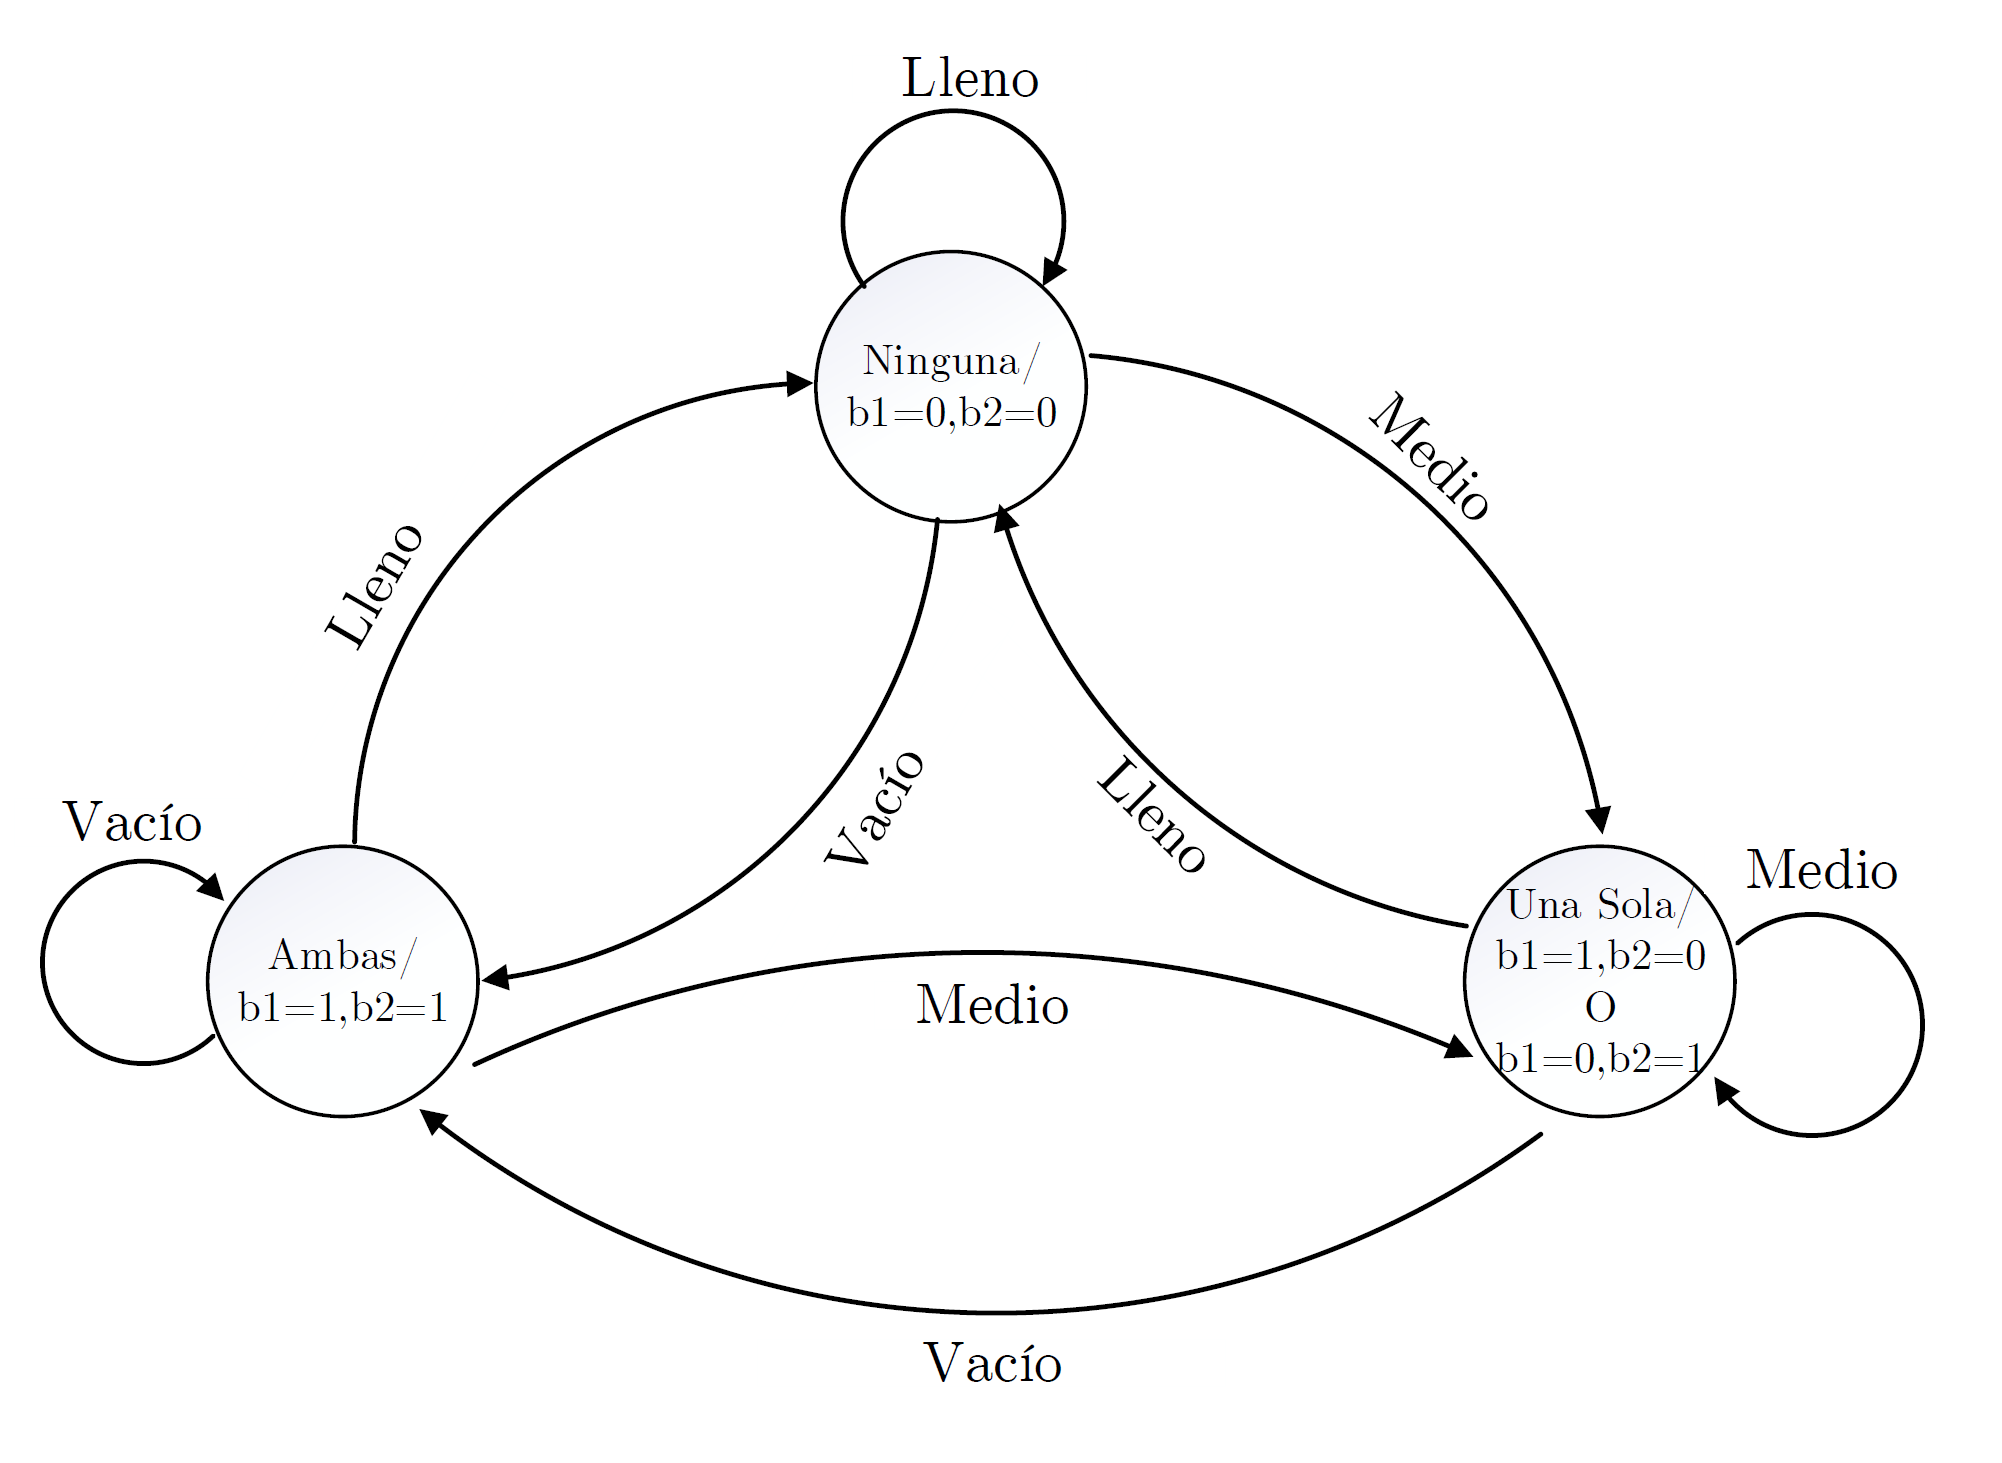
\includegraphics[scale=0.4]{images/diagrama_estados_moore.png}
\caption{Diagrama de estados y transiciones} \label{1_figa}
\end{figure}

Al contar con 3 estados diferentes, mi maquina de estados necesitará como mínimo dos Flip-Flop's para almacenar el estado actual. Los tres estados posibles se codifican a traves de dos variables $y_1$ e $y_0$, de esta forma, tendremos las siguientes configuraciones:

\bigskip

\begin{table}[ht]
	\centering
	\begin{tabular}{c|c}
	Estado & $y_1y_0$ \\ 
	\hline 
	Ninguna & 00 \\ 
	Una Sola & 01 \\ 
	Ambas & 11 \\ 
	\end{tabular} 
\end{table}


Habiendo definido los estados del diseño, se procedió a completar la correspondiente tabla de asignación de estados:
\bigskip
\begin{table}[ht]
	\centering
	\begin{tabular}{c|c|c|c|c}
	Estado Actual & \multicolumn{3}{c|}{Próximo Estado$(Y_1Y_0)$} & Salida\\
	\cline{2-4}
	$(y_1y_0)$ & $SI=00$ & $SI=01$ & $SI=11$ & $(b_1b_2)$\\
	\hline
	00 & 11 & 01 & 00 & 00 \\
	01 & 11 & 01 & 00 & 01 o 10 (Alternado) \\
	11 & 11 & 01 & 00 & 11 \\
	\end{tabular}
	\caption{Tabla de asignación de estados}
	\label{1_t1}
\end{table}

A partir del Cuadro \ref{1_t1} se confeccionó el Cuadro \ref{1_t2}, que implementa la tabla de verdad que determina el próximo estado ($Y_1Y_0$) en función del estado anterior ($y_1y_0$) y las entradas ($SI$). 



\begin{table}[H]
	\centering
	\begin{tabular}{c|c|c}
	$y_1y_0SI$ & $Y_1$ & $Y_0$  \\ 
	\hline 
	0000 & 1 & 1  \\ 
	\hline 
	0001 & 0 & 1  \\ 
	\hline 
	0010 & x & x  \\ 
	\hline 
	0011 & 0 & 0  \\ 
	\hline 
	0100 & 1 & 1  \\ 
	\hline 
	0101 & 0 & 1  \\ 
	\hline 
	0110 & x & x  \\ 
	\hline 
	0111 & 0 & 0  \\ 
	\hline 
	1000 & x & x  \\ 
	\hline 
	1001 & x & x  \\ 
	\hline 
	1010 & x & x  \\ 
	\hline 
	1011 & x & x  \\ 
	\hline 
	1100 & 1 & 1  \\ 
	\hline 
	1101 & 0 & 1  \\ 
	\hline 
	1110 & x & x  \\ 
	\hline 
	1111 & 0 & 0  \\ 
	\end{tabular} 
	\caption{Tabla de verdad cambio de estado}
	\label{1_t2}
\end{table}

Se determinó que es estado $SI=10$ no es una combinación posible, ya que indicaría que el agua ha superado el sensor superior pero no el inferior, lo cual es incompatible con el modelo del deposito, e indicaría un error en los sensores. Como el manejo de errores en el sensores excede los requisitos de la consigna es que se determinó que no son combinaciones posibles y las salidas correspondientes a estas configuraciones se determinaron como 'don't care'

La simplificación mediante Mapas de Karnaugh arrojó los siguientes resultados:

\[
Y_1 = \overline{S}.\overline{I} = \overline{I+S}
\]

\[
Y_0 = \overline{S} = \overline{S + S}
\]

Se observa que el 'próximo estado' no depende del estado actual, sino solamente de las entradas. Se escriben como una negación de suma para luego implementar mediante una compuerta NOR.



\subsection*{Implementación}
\begin{figure}[H]
\centering
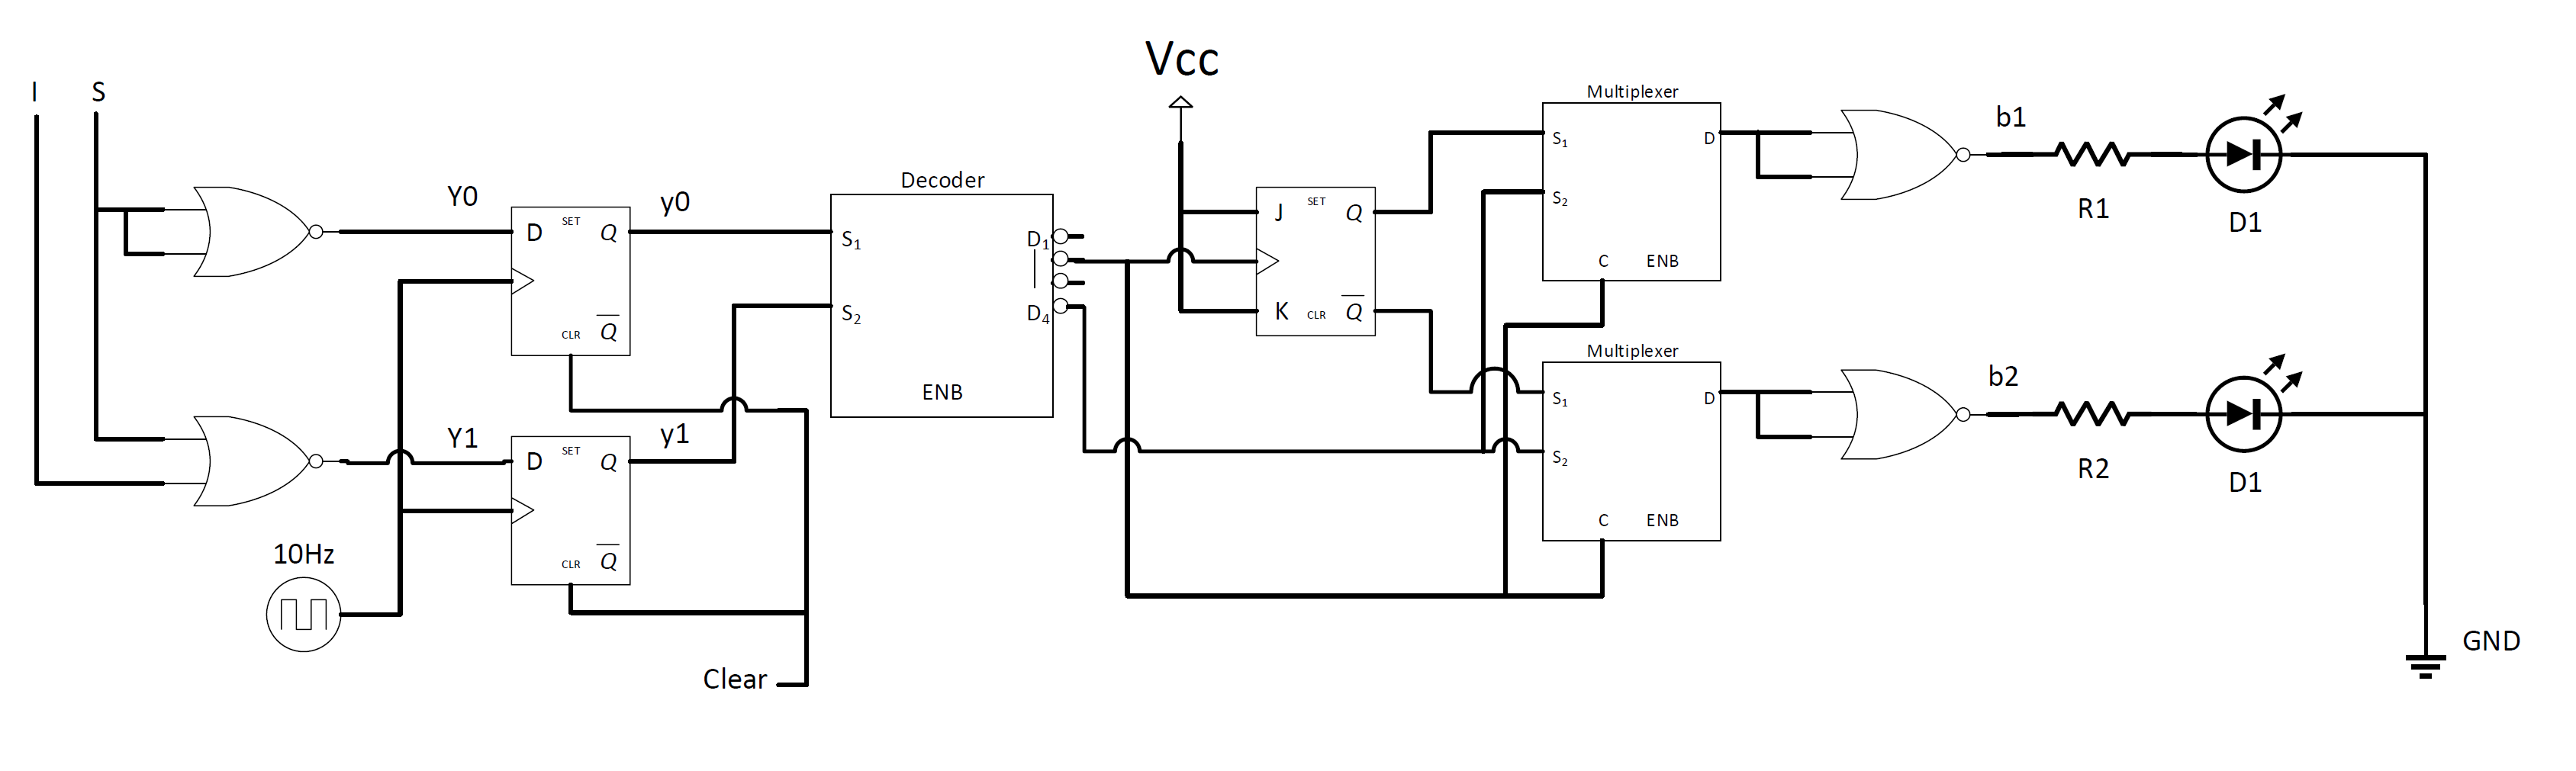
\includegraphics[scale=0.42]{images/diagrama_moore.png}
\caption{Diagrama Esquemático de la Máquina de Estados}
\label{1_fig2}
\end{figure}

La Figura \ref{1_fig2} muestra el circuito implementado. Las salidas de los Flip-Flop's D almacenan el estado actual de la maquina de de estados, mientras que toda la lógica a la salida de estos Flip-Flop's controla las salidas de la máquina.  Se implementó un Flip-Flop JK en modo Toggle para alternar la activación de las bombas cuando solo una de ellas debe activarse. Como se observa, el clock de este Flip-Flop esta controlado por la señal $\overline{Uno Solo}$, la cual valdrá 0 cuando la máquina se encuentre en el estado 'Uno Solo' y valdrá 1 en caso contrario. Cada vez que se produzca una transición del estado 'Uno Solo' hacia otro estado, se invertirán las salidas del Flip-Flop JK. Las salidas $Q$ y $\overline{Q}$ de este Flip-Flop sirven a una de dos entradas de dos multiplexores distintos. La entrada restante esta alimentada por la señal $\overline{Ambas}$, la cual valdrá 0 cuando la máquina se encuentre en el estado 'Ambas'. La señal de selección de ambos multiplexores está controlada por la señal $\overline{Una Sola}$, presentada anteriormente. Así se logra que se alternen las bombas cuando solo una debe encenderse y que se enciendan o apaguen ambas juntas cuando corresponda. Lo que sucede es que la linea de selección de los multiplexores determinan si las bombas tienen el mismo estado o estados complementarios.

\section*{Implementación Maquina de Mealy}
\subsection*{Diagrama de Estados y Transiciones}
Al igual que en el proceso de diseño de la máquina de estados de Moore, el primer paso fue determinar los estados 

\end{document}
\documentclass[10pt,a4paper]{article}
\usepackage{tikz}
\usetikzlibrary{matrix,calc}
\usepackage{multirow}
\usepackage[utf8]{inputenc}
\usepackage[spanish]{babel}
\usepackage{amsmath}
\usepackage{amsfonts}
\usepackage{amssymb}
\usepackage{graphicx}
\usepackage{float}
\usepackage[left=2cm,right=2cm,top=2cm,bottom=2cm]{geometry}
\usepackage{circuitikz}
\usepackage{tikz-timing}
\usetikztiminglibrary[rising arrows]{clockarrows}
\usepackage{pgfplots}
\pgfplotsset{compat=1.15}
\usepackage{listings}
\usepackage[export]{adjustbox}
\usepackage{graphicx,wrapfig,lipsum}
\usepackage{booktabs}
\usepackage[skip=0pt]{caption}
\usepackage{pdfpages}
\captionsetup[figure]{font=small,labelfont=small}


\usetikzlibrary{matrix,calc}

%isolated term
%#1 - Optional. Space between node and grouping line. Default=0
%#2 - node
%#3 - filling color
\newcommand{\implicantsol}[3][0]{
    \draw[rounded corners=3pt, fill=#3, opacity=0.3] ($(#2.north west)+(135:#1)$) rectangle ($(#2.south east)+(-45:#1)$);
    }


%internal group
%#1 - Optional. Space between node and grouping line. Default=0
%#2 - top left node
%#3 - bottom right node
%#4 - filling color
\newcommand{\implicant}[4][0]{
    \draw[rounded corners=3pt, fill=#4, opacity=0.3] ($(#2.north west)+(135:#1)$) rectangle ($(#3.south east)+(-45:#1)$);
    }

%group lateral borders
%#1 - Optional. Space between node and grouping line. Default=0
%#2 - top left node
%#3 - bottom right node
%#4 - filling color
\newcommand{\implicantcostats}[4][0]{
    \draw[rounded corners=3pt, fill=#4, opacity=0.3] ($(rf.east |- #2.north)+(90:#1)$)-| ($(#2.east)+(0:#1)$) |- ($(rf.east |- #3.south)+(-90:#1)$);
    \draw[rounded corners=3pt, fill=#4, opacity=0.3] ($(cf.west |- #2.north)+(90:#1)$) -| ($(#3.west)+(180:#1)$) |- ($(cf.west |- #3.south)+(-90:#1)$);
}

%group top-bottom borders
%#1 - Optional. Space between node and grouping line. Default=0
%#2 - top left node
%#3 - bottom right node
%#4 - filling color
\newcommand{\implicantdaltbaix}[4][0]{
    \draw[rounded corners=3pt, fill=#4, opacity=0.3] ($(cf.south -| #2.west)+(180:#1)$) |- ($(#2.south)+(-90:#1)$) -| ($(cf.south -| #3.east)+(0:#1)$);
    \draw[rounded corners=3pt, fill=#4, opacity=0.3] ($(rf.north -| #2.west)+(180:#1)$) |- ($(#3.north)+(90:#1)$) -| ($(rf.north -| #3.east)+(0:#1)$);
}

%group corners
%#1 - Optional. Space between node and grouping line. Default=0
%#2 - filling color
\newcommand{\implicantcantons}[2][0]{
    \draw[rounded corners=3pt, opacity=.3] ($(rf.east |- 0.south)+(-90:#1)$) -| ($(0.east |- cf.south)+(0:#1)$);
    \draw[rounded corners=3pt, opacity=.3] ($(rf.east |- 8.north)+(90:#1)$) -| ($(8.east |- rf.north)+(0:#1)$);
    \draw[rounded corners=3pt, opacity=.3] ($(cf.west |- 2.south)+(-90:#1)$) -| ($(2.west |- cf.south)+(180:#1)$);
    \draw[rounded corners=3pt, opacity=.3] ($(cf.west |- 10.north)+(90:#1)$) -| ($(10.west |- rf.north)+(180:#1)$);
    \fill[rounded corners=3pt, fill=#2, opacity=.3] ($(rf.east |- 0.south)+(-90:#1)$) -|  ($(0.east |- cf.south)+(0:#1)$) [sharp corners] ($(rf.east |- 0.south)+(-90:#1)$) |-  ($(0.east |- cf.south)+(0:#1)$) ;
    \fill[rounded corners=3pt, fill=#2, opacity=.3] ($(rf.east |- 8.north)+(90:#1)$) -| ($(8.east |- rf.north)+(0:#1)$) [sharp corners] ($(rf.east |- 8.north)+(90:#1)$) |- ($(8.east |- rf.north)+(0:#1)$) ;
    \fill[rounded corners=3pt, fill=#2, opacity=.3] ($(cf.west |- 2.south)+(-90:#1)$) -| ($(2.west |- cf.south)+(180:#1)$) [sharp corners]($(cf.west |- 2.south)+(-90:#1)$) |- ($(2.west |- cf.south)+(180:#1)$) ;
    \fill[rounded corners=3pt, fill=#2, opacity=.3] ($(cf.west |- 10.north)+(90:#1)$) -| ($(10.west |- rf.north)+(180:#1)$) [sharp corners] ($(cf.west |- 10.north)+(90:#1)$) |- ($(10.west |- rf.north)+(180:#1)$) ;
}

%Empty Karnaugh map 4x4
\newenvironment{Karnaugh}%
{
\begin{tikzpicture}[baseline=(current bounding box.north),scale=0.8]
\draw (0,0) grid (4,4);
\draw (0,4) -- node [pos=0.7,above right,anchor=south west] {cd} node [pos=0.7,below left,anchor=north east] {ab} ++(135:1);
%
\matrix (mapa) [matrix of nodes,
        column sep={0.8cm,between origins},
        row sep={0.8cm,between origins},
        every node/.style={minimum size=0.3mm},
        anchor=8.center,
        ampersand replacement=\&] at (0.5,0.5)
{
                       \& |(c00)| 00         \& |(c01)| 01         \& |(c11)| 11         \& |(c10)| 10         \& |(cf)| \phantom{00} \\
|(r00)| 00             \& |(0)|  \phantom{0} \& |(1)|  \phantom{0} \& |(3)|  \phantom{0} \& |(2)|  \phantom{0} \&                     \\
|(r01)| 01             \& |(4)|  \phantom{0} \& |(5)|  \phantom{0} \& |(7)|  \phantom{0} \& |(6)|  \phantom{0} \&                     \\
|(r11)| 11             \& |(12)| \phantom{0} \& |(13)| \phantom{0} \& |(15)| \phantom{0} \& |(14)| \phantom{0} \&                     \\
|(r10)| 10             \& |(8)|  \phantom{0} \& |(9)|  \phantom{0} \& |(11)| \phantom{0} \& |(10)| \phantom{0} \&                     \\
|(rf) | \phantom{00}   \&                    \&                    \&                    \&                    \&                     \\
};
}%
{
\end{tikzpicture}
}

%Empty Karnaugh map 2x4
\newenvironment{Karnaughvuit}%
{
\begin{tikzpicture}[baseline=(current bounding box.north),scale=0.8]
\draw (0,0) grid (4,2);
\draw (0,2) -- node [pos=0.7,above right,anchor=south west] {bc} node [pos=0.7,below left,anchor=north east] {a} ++(135:1);
%
\matrix (mapa) [matrix of nodes,
        column sep={0.8cm,between origins},
        row sep={0.8cm,between origins},
        every node/.style={minimum size=0.3mm},
        anchor=4.center,
        ampersand replacement=\&] at (0.5,0.5)
{
                      \& |(c00)| 00         \& |(c01)| 01         \& |(c11)| 11         \& |(c10)| 10         \& |(cf)| \phantom{00} \\
|(r00)| 0             \& |(0)|  \phantom{0} \& |(1)|  \phantom{0} \& |(3)|  \phantom{0} \& |(2)|  \phantom{0} \&                     \\
|(r01)| 1             \& |(4)|  \phantom{0} \& |(5)|  \phantom{0} \& |(7)|  \phantom{0} \& |(6)|  \phantom{0} \&                     \\
|(rf) | \phantom{00}  \&                    \&                    \&                    \&                    \&                     \\
};
}%
{
\end{tikzpicture}
}

%Empty Karnaugh map 2x2
\newenvironment{Karnaughquatre}%
{
\begin{tikzpicture}[baseline=(current bounding box.north),scale=0.8]
\draw (0,0) grid (2,2);
\draw (0,2) -- node [pos=0.7,above right,anchor=south west] {b} node [pos=0.7,below left,anchor=north east] {a} ++(135:1);
%
\matrix (mapa) [matrix of nodes,
        column sep={0.8cm,between origins},
        row sep={0.8cm,between origins},
        every node/.style={minimum size=0.3mm},
        anchor=2.center,
        ampersand replacement=\&] at (0.5,0.5)
{
          \& |(c00)| 0          \& |(c01)| 1  \\
|(r00)| 0 \& |(0)|  \phantom{0} \& |(1)|  \phantom{0} \\
|(r01)| 1 \& |(2)|  \phantom{0} \& |(3)|  \phantom{0} \\
};
}%
{
\end{tikzpicture}
}

%Defines 8 or 16 values (0,1,X)
\newcommand{\contingut}[1]{%
\foreach \x [count=\xi from 0]  in {#1}
     \path (\xi) node {\x};
}

%Places 1 in listed positions
\newcommand{\minterms}[1]{%
    \foreach \x in {#1}
        \path (\x) node {1};
}

%Places 0 in listed positions
\newcommand{\maxterms}[1]{%
    \foreach \x in {#1}
        \path (\x) node {0};
}

%Places X in listed positions
\newcommand{\indeterminats}[1]{%
    \foreach \x in {#1}
        \path (\x) node {X};
}
\newenvironment{KarnaughTP3}%
{
\begin{tikzpicture}[baseline=(current bounding box.north),scale=0.8]
\draw (0,0) grid (4,4);
\draw (0,4) -- node [pos=0.9,above right,anchor=south west] {$Q_1 Q_0$} node [pos=0.7,below left,anchor=north east] {$W Q_2$} ++(135:1);
%
\matrix (mapa) [matrix of nodes,
        column sep={0.8cm,between origins},
        row sep={0.8cm,between origins},
        every node/.style={minimum size=0.3mm},
        anchor=8.center,
        ampersand replacement=\&] at (0.5,0.5)
{
                       \& |(c00)| 00         \& |(c01)| 01         \& |(c11)| 11         \& |(c10)| 10         \& |(cf)| \phantom{00} \\
|(r00)| 00             \& |(0)|  \phantom{0} \& |(1)|  \phantom{0} \& |(3)|  \phantom{0} \& |(2)|  \phantom{0} \&                     \\
|(r01)| 01             \& |(4)|  \phantom{0} \& |(5)|  \phantom{0} \& |(7)|  \phantom{0} \& |(6)|  \phantom{0} \&                     \\
|(r11)| 11             \& |(12)| \phantom{0} \& |(13)| \phantom{0} \& |(15)| \phantom{0} \& |(14)| \phantom{0} \&                     \\
|(r10)| 10             \& |(8)|  \phantom{0} \& |(9)|  \phantom{0} \& |(11)| \phantom{0} \& |(10)| \phantom{0} \&                     \\
|(rf) | \phantom{00}   \&                    \&                    \&                    \&                    \&                     \\
};
}%
{
\end{tikzpicture}
}

\newenvironment{KarnaughvuiteTP3}%
{
\begin{tikzpicture}[baseline=(current bounding box.north),scale=0.8]
\draw (0,0) grid (4,2);
\draw (0,2) -- node [pos=0.9,above right,anchor=south west] {$Q_1Q_0$} node [pos=0.7,below left,anchor=north east] {$W$} ++(135:1);
%
\matrix (mapa) [matrix of nodes,
        column sep={0.8cm,between origins},
        row sep={0.8cm,between origins},
        every node/.style={minimum size=0.3mm},
        anchor=4.center,
        ampersand replacement=\&] at (0.5,0.5)
{
                      \& |(c00)| 00         \& |(c01)| 01         \& |(c11)| 11         \& |(c10)| 10         \& |(cf)| \phantom{00} \\
|(r00)| 0             \& |(0)|  \phantom{0} \& |(1)|  \phantom{0} \& |(3)|  \phantom{0} \& |(2)|  \phantom{0} \&                     \\
|(r01)| 1             \& |(4)|  \phantom{0} \& |(5)|  \phantom{0} \& |(7)|  \phantom{0} \& |(6)|  \phantom{0} \&                     \\
|(rf) | \phantom{00}  \&                    \&                    \&                    \&                    \&                     \\
};
}%
{
\end{tikzpicture}
}

\begin{document}
\section*{Ejercicio 2}

\subsection*{Moore}
Se nos pidi\'o realizar una m\'aquina de Moore y una de Mealy que puedan detectar la secuencia 1-1-0-1 y avise en la salida al detectarla. Para esto tuvimos en cuenta que cuando termina la secuencia y es detectada se toma el \'ultimo 1 de la secuencia como el primero de la siguiente secuencia en caso de que ocurran 2 secuencias seguidas, la cual ser\'ia 1-1-0-1-1-0-1. Primero diseñamos un diagrama de estados basándonos en la m\'aquina de Moore, donde tendremos 5 estados. El estado A es el caso base donde se recibió un 0 fuera de la secuencia pedida, el estado B es el caso donde se recibió el primer 1, el estado C es el caso donde se recibe el segundo 1, el estado D donde se recibe la secuencia 1-1-0 y el estado E es cuando se recibe la secuencia completa. 
El diagrama queda de la siguiente manera:

\begin{figure}[hbtp]
	\centering
		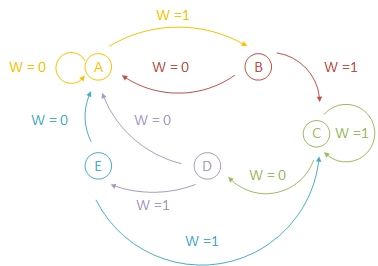
\includegraphics[scale=1]{Imagenes/diagestmoore.jpg}
	\caption{Diagrama de Estados - Máquina de Moore}
	\label{2_fig0}
\end{figure}

Se le otorgó a cada estado un valor representativo en binario, siendo el estado A un 0 y el estado E un 6 (el cual al estar en binario se representara como 1-1-0), no utilizamos los valores comunes del 0 al 4 ya que preferimos utilizar el código de Grey para que los flip flops tuvieran menos transiciones al pasar de un estado al otro. Como el estado E es un número que necesita 3 bits de memoria, se utilizar\'an 3 flip flop para almacenar el número del estado actual, cada flip flop se representar\'a en este ejercicio como $Q_n$, siendo entonces cada uno representación de un bit del estado en el cual se encuentra el circuito. El flip flop $Q_0$ representa el bit menos significativo, y el $Q_2$ el bit más significativo. Cada estado podr\'a pasar a otro seg\'un la entrada que reciba, como se mostró en el diagrama anterior, ahora pasamos a representar el esquema en una tabla con las variaciones de los estados:

\begin{figure}[H]
	\begin{center}
		\begin{tabular}{c|c|c|c|}
		\cline{2-4}
		\textbf{} & \textbf{W = 0} & \textbf{W = 1} & \textbf{Z} \\ \hline
		\multicolumn{1}{|c|}{\textbf{A$_{000}$}} & \textbf{A} & \textbf{B} & \textbf{0} \\ \hline
		\multicolumn{1}{|c|}{\textbf{B$_{001}$}} & \textbf{A} & \textbf{C} & \textbf{0} \\ \hline
		\multicolumn{1}{|c|}{\textbf{C$_{011}$}} & \textbf{D} & \textbf{A} & \textbf{0} \\ \hline
		\multicolumn{1}{|c|}{\textbf{D$_{010}$}} & \textbf{A} & \textbf{E} & \textbf{0} \\ \hline
		\multicolumn{1}{|c|}{\textbf{E$_{110}$}} & \textbf{A} & \textbf{C} & \textbf{1} \\ \hline
		\end{tabular}
	\caption{Transiciones con Estados - Máquina de Moore} 
	\label{2_fig1}
	\end{center}
\end{figure}
Si ahora representamos a cada estado con sus respectivos valores $Q_n$ para ver las transiciones la tabla quedar\'a con valores 1 y 0 que representar\'an una salida High o Low respectivamente. As\'i podremos analizar cada flip flop por separado y llegar a un circuito combinacional que los alimente, para esto tenemos que discriminar entre los estados actuales $Q{n_{t}}$ y los estados siguientes $Q{n_{t+1}}$. La tabla dicha es la siguiente:


\begin{figure}[H]
	\begin{center}
		\begin{tabular}{|c|c|c|c|c|c|c|c|c|c|}
\hline
\multicolumn{3}{|c|}{\multirow{2}{*}{\textbf{Estado Actual}}} & \multicolumn{6}{c|}{\textbf{Estado}} & \multirow{2}{*}{\textbf{Salida}} \\ \cline{4-9}
\multicolumn{3}{|c|}{} & \multicolumn{3}{c|}{\textbf{W = 0}} & \multicolumn{3}{c|}{\textbf{W = 1}} &  \\ \hline
\textbf{$Q_{2_{t}}$} & \textbf{$Q_{1_{t}}$} & \textbf{$Q_{0_{t}}$} & \textbf{$Q_{2_{t+1}}$} & \textbf{$Q_{1_{t+1}}$} & \textbf{$Q_{0_{t+1}}$} & \textbf{$Q_{2_{t+1}}$} & \textbf{$Q_{1_{t+1}}$} & \textbf{$Q_{0_{t+1}}$} & \textbf{Z} \\ \hline
\textbf{0} & \textbf{0} & \textbf{0} & \textbf{0} & \textbf{0} & \textbf{0} & \textbf{0} & \textbf{0} & \textbf{1} & \textbf{0} \\ \hline
\textbf{0} & \textbf{0} & \textbf{1} & \textbf{0} & \textbf{0} & \textbf{0} & \textbf{0} & \textbf{1} & \textbf{1} & \textbf{0} \\ \hline
\textbf{0} & \textbf{1} & \textbf{1} & \textbf{0} & \textbf{1} & \textbf{0} & \textbf{0} & \textbf{1} & \textbf{1} & \textbf{0} \\ \hline
\textbf{0} & \textbf{1} & \textbf{0} & \textbf{0} & \textbf{0} & \textbf{0} & \textbf{1} & \textbf{1} & \textbf{0} & \textbf{0} \\ \hline
\textbf{1} & \textbf{1} & \textbf{0} & \textbf{0} & \textbf{0} & \textbf{0} & \textbf{0} & \textbf{1} & \textbf{1} & \textbf{1} \\ \hline
\textbf{1} & \textbf{1} & \textbf{1} & \textbf{X} & \textbf{X} & \textbf{X} & \textbf{X} & \textbf{X} & \textbf{X} & \textbf{X} \\ \hline
\textbf{1} & \textbf{0} & \textbf{1} & \textbf{X} & \textbf{X} & \textbf{X} & \textbf{X} & \textbf{X} & \textbf{X} & \textbf{X} \\ \hline
\textbf{1} & \textbf{0} & \textbf{0} & \textbf{X} & \textbf{X} & \textbf{X} & \textbf{X} & \textbf{X} & \textbf{X} & \textbf{X} \\ \hline
		\end{tabular}
		\caption{Transiciones con Flip Flop - Máquina de Moore} 
		\label{2_fig2}
	\end{center}
\end{figure}

Para analizar esta tabla debemos tener en cuenta que para la máquina de Moore los estados son dependientes de las entradas y de ellos mismos, por lo que cada estado $Q_{n_{t}}$ depender\'a tanto de la entrada $W$ como de los estados $Q_{2_{t}}$,$Q_{1_{t}}$ y $Q_{0_{t}}$. Mientras que la salida $Z$ depende solo de los estados $Q_{2_{t}}$, $Q_{1_{t}}$ y $Q_{0_{t}}$. Por lo que pasaremos a analizar cada columna $Q_{n_{t+1}}$ dependiendo de cada combinaci\'on $Q{n_{t}}$ y la entrada $W$, y luego analizaremos la columna $Z$ para cada combinaci\'on de los $Q{n_{t}}$. Para analizar las columnas las resolvimos con mapas de Karnaugh para simplificar más rápido los minit\'erminos quedando los estados y la salida de las siguientes maneras:
	
\begin{figure}[H]
	\begin{center}
	\begin{KarnaughTP3}
	\contingut{0,0,0,0,X,X,0,X,1,1,0,1,X,X,1,X}
	\implicant{12}{14}{red}
	\implicant{12}{9}{blue}
	\implicant{13}{11}{green}
	\end{KarnaughTP3}
	\end{center}
	\caption{$Q_{0_{t+1}}$ Máq. de Moore} 
	\label{2_fig3}
\end{figure}

\begin{figure}[H]
	\begin{center}
		\begin{KarnaughTP3}
		\contingut{0,0,0,1,X,X,0,X,0,1,1,1,X,X,1,X}
		\implicant{12}{14}{orange}
		\implicant{13}{11}{green}
		\implicant{3}{11}{red}
		\implicant{15}{10}{blue}
		\end{KarnaughTP3}
	\end{center}
	\caption{$Q_{1_{t+1}}$ Máq. de Moore} 
	\label{2_fig4}
\end{figure}

\begin{figure}[H]
	\begin{center}
		\begin{KarnaughTP3}
		\contingut{0,0,0,0,X,X,0,X,0,0,1,0,X,X,0,X}
		\implicant{10}{10}{red}
		\end{KarnaughTP3}
	\end{center}
	\caption{$Q_{2_{t+1}}$ Máq. de Moore} 
	\label{2_fig5}
\end{figure}
	
\begin{figure}[H]
	\begin{center}
		\begin{KarnaughvuiteQ2TP3}
		\minterms{6}
		\maxterms{0,1,2,3}
		\indeterminats{5,4,7}
		\implicant{4}{6}{orange}
		\end{KarnaughvuiteQ2TP3}
	\end{center}
	\caption{$Z$: Salida - Máq. de Moore} 
	\label{2_fig6}
\end{figure}

Tomando las agrupaciones marcadas en cada mapa podemos formas las ecuaciones que representarán a  $Q_{0_{t+1}}, Q_{1_{t+1}}, Q_{2_{t+1}}$ y $Z$ respectivamente, quedando las ecuaciones de la siguiente manera:

\begin{align*}
	Q_{0_{t+1}} &= W * \overline{Q_{1}} + W * ( Q_{2} + Q_{0} ) \\
	Q_{1_{t+1}} &= W * ( Q_{2} + Q_{0} ) + Q_{1} * ( W + Q_{0} ) \\
	Q_{2_{t+1}} &= W * \overline{Q_{2}} * Q_{1} * \overline{Q_{0}} \\
	Z &= Q_{2} \\
\end{align*}
Una vez que ya tenemos las ecuaciones procedemos a armar el circuito:

\begin{figure}[H]
\centering
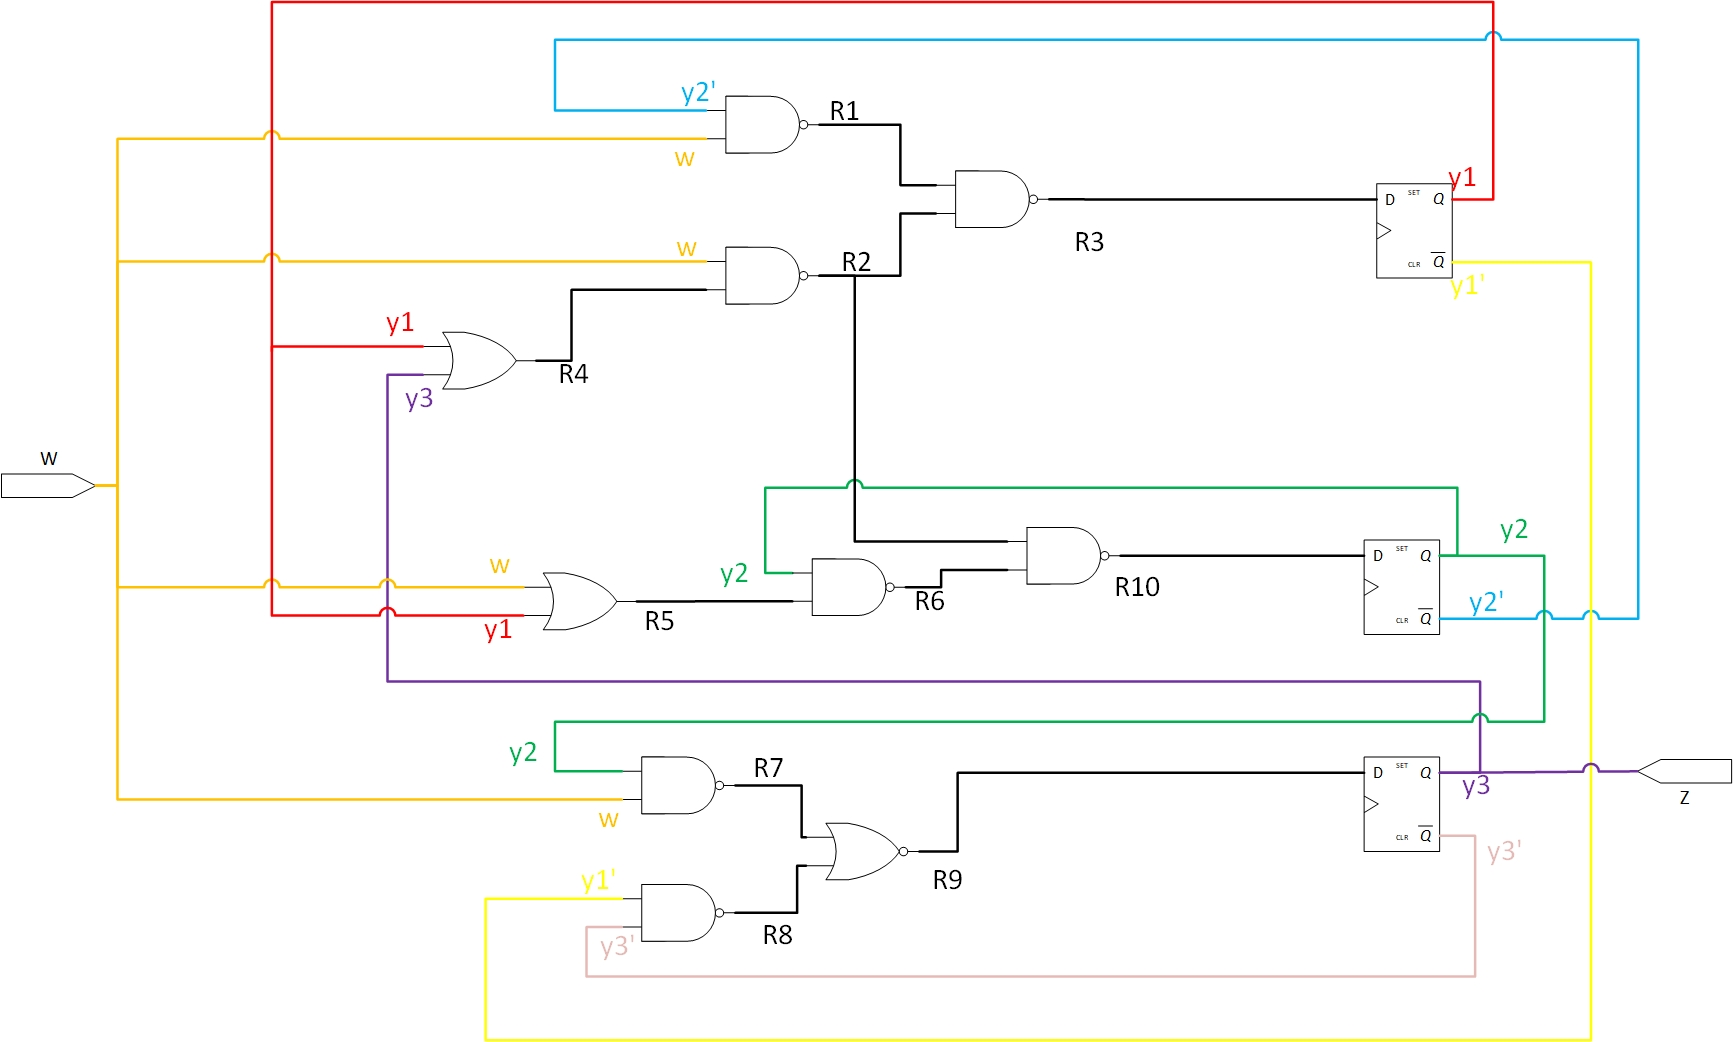
\includegraphics[width=14cm]{Imagenes/TP2_EJ2_MOORE_GREY.jpg}
\caption{Circuito lógico de Moore}
\end{figure}

%%%%				VERILOOOOOOG



Pudimos observar que el circuito encuentra bien la secuencia pedida.

\subsection*{Mealy}

También se nos pidi\'o armar una m\'aquina pero de Mealy en lugar de Moore. Para esto rediseñamos el diagrama de la máquina de estados utilizando la notaci\'on de Mealy con flechas que indiquen la entrada y la salida entre transición de estados. Utilizando este método tendremos menos estados pero la salida esta vez será dependiente tanto de los estados como de las entradas.

\begin{figure}[H]
	\centering
	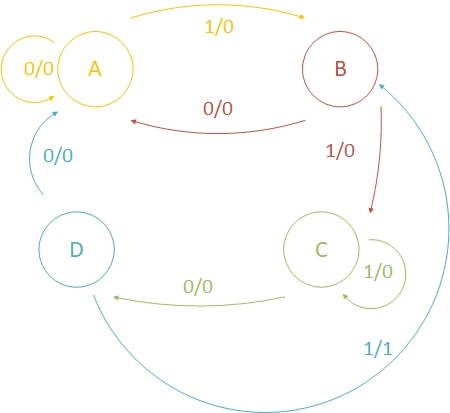
\includegraphics[scale=0.6]{Imagenes/diagestmealy.jpg}
	\caption{Diagrama de Estados - Máquina de Mealy}
	\label{2_fig7}
\end{figure}

Partiendo de este nuevo diagrama, se tabula un nuevo cuadro con la transiciones de estados y la salida, para luego asignarle un valor numérico a cada estado. Como esta vez son 4 estados solo se necesitara representar desde el 0 al 3, los cuales en binario serán 0-0 y 1-1, solo se necesitaran 2 flip flops para esta máquina de estados. La siguiente tabla muestra los valores que $Q_{1_{t+1}}$ $Q_{0_{t+1}}$ y $Z$ tendrán ahora.

\begin{figure}[H]
	\begin{center}
		\begin{tabular}{|c|c|c|c|c|}
\hline
\multirow{2}{*}{\textbf{\begin{tabular}[c]{@{}c@{}}Estado\\ Actual\end{tabular}}} & \multicolumn{2}{c|}{\textbf{\begin{tabular}[c]{@{}c@{}}Estado\\ Siguiente\end{tabular}}} & \multicolumn{2}{c|}{\textbf{Salida: Z}} \\ \cline{2-5} 
 & \textbf{W = 0} & \textbf{W = 1} & \textbf{W = 0} & \textbf{W = 1} \\ \hline
\textbf{A$_{000}$} & \textbf{A} & \textbf{B} & \textbf{0} & \textbf{0} \\ \hline
\textbf{B$_{001}$} & \textbf{A} & \textbf{C} & \textbf{0} & \textbf{0} \\ \hline
\textbf{C$_{010}$} & \textbf{D} & \textbf{C} & \textbf{0} & \textbf{0} \\ \hline
\textbf{D$_{011}$} & \textbf{A} & \textbf{B} & \textbf{0} & \textbf{1} \\ \hline
		\end{tabular}
	\caption{Transiciones - Máquina de Mealy} 
	\label{2_fig8}
	\end{center}
\end{figure}


En este caso hicimos un análisis previo y decidimos ordenar los estados por código de Grey para q de un estado a otro solo haya un cambio de estado, solo un bit cambiaría entre cada transición excepto del estado C al A, lo que significaría que un solo flip flop cambiaría entre estado. Siendo entonces el estado A la combinación 0-0, B la combinación 0-1, C la combinación 1-1 y por último D la combinación 1-0. Utilizamos este método ya que nos ahorraba un integrado a comparación del anterior. La siguiente tabla muestra las transiciones con el código de Grey:


\begin{figure}[H]
	\begin{center}
		\begin{tabular}{|c|c|c|c|c|c|c|c|}
\hline
\multicolumn{2}{|c|}{\multirow{2}{*}{\textbf{\begin{tabular}[c]{@{}c@{}}Estado\\ Actual\end{tabular}}}} & \multicolumn{4}{c|}{\textbf{Estado Siguiente}} & \multicolumn{2}{c|}{\multirow{2}{*}{\textbf{Salida: Z}}} \\ \cline{3-6}
\multicolumn{2}{|c|}{} & \multicolumn{2}{c|}{\textbf{W = 0}} & \multicolumn{2}{c|}{\textbf{W = 1}} & \multicolumn{2}{c|}{} \\ \hline
\textbf{$Q_{1_{t}}$} & \textbf{$Q_{0_{t}}$} & \textbf{$Q_{1_{t+1}}$} & \textbf{$Q_{0_{t+1}}$} & \textbf{$Q_{1_{t+1}}$} & \textbf{$Q_{0_{t+1}}$} & \textbf{W = 0} & \textbf{W = 1} \\ \hline
\textbf{0} & \textbf{0} & \textbf{0} & \textbf{0} & \textbf{0} & \textbf{1} & \textbf{0} & \textbf{0} \\ \hline
\textbf{0} & \textbf{1} & \textbf{0} & \textbf{0} & \textbf{1} & \textbf{1} & \textbf{0} & \textbf{0} \\ \hline
\textbf{1} & \textbf{1} & \textbf{1} & \textbf{0} & \textbf{1} & \textbf{1} & \textbf{0} & \textbf{0} \\ \hline
\textbf{1} & \textbf{0} & \textbf{0} & \textbf{0} & \textbf{0} & \textbf{1} & \textbf{0} & \textbf{1} \\ \hline
		\end{tabular}
	\caption{Transiciones con Flip Flop - Máquina de Mealy} 
	\label{2_fig9}
	\end{center}
\end{figure}

Teniendo en cuenta que la única diferencia en esta parte con respecto a Moore es que la salida $Z$ depende de la entrada y los estados, pasamos a analizar las columnas de la tabla anterior. Las resolvimos con mapas de Karnaugh para simplificar más rápido los minit\'erminos quedando los estados y la salida de las siguientes maneras:

\begin{figure}[H]
	\begin{center}
		\begin{KarnaughvuiteTP3}
		\minterms{4,5,6,7}
		\maxterms{0,1,2,3}
		%\indeterminats{2,5}
		\implicant{4}{6}{green}
		\end{KarnaughvuiteTP3}
	\end{center}
	\caption{$Q_{0_{t+1}}$ Máq. de Mealy} 
	\label{2_fig10}
\end{figure}

\begin{figure}[H]
	\begin{center}
		\begin{KarnaughvuiteTP3}	
		\minterms{3,5,7}
		\maxterms{0,1,2,4,6}
		%\indeterminats{2,5}
		\implicant{3}{7}{green}
		\implicant{5}{7}{red}
		\end{KarnaughvuiteTP3}
	\end{center}
	\caption{$Q_{1_{t+1}}$ Máq. de Mealy} 
	\label{2_fig11}
\end{figure}
	
\begin{figure}[H]
	\begin{center}
		\begin{KarnaughvuiteTP3}
		\minterms{6}
		\maxterms{0,1,2,3,4,5,7}
		%\indeterminats{2,5}
		\implicant{6}{6}{green}
		\end{KarnaughvuiteTP3}
	\end{center}
	\caption{$Z$: Salida - Máq. de Mealy} 
	\label{2_fig12}
\end{figure}

Tomando las agrupaciones marcadas en cada mapa podemos formas las ecuaciones que representarán a  $Q_{0_{t+1}}, Q_{1_{t+1}}, Q_{2_{t+1}}$ y $Z$ respectivamente, quedando las ecuaciones de la siguiente manera:

\begin{align*}
	Q_{0_{t+1}} &= W  \\
	Q_{1_{t+1}} &= Q_{0} * ( Q_{1} + w ) \\
	Z &= w * Q_{1} * \overline{Q_{0}} \\
\end{align*}
De estas ecuaciones podemos formar el siguiente circuito:

\begin{figure}[H]
\centering
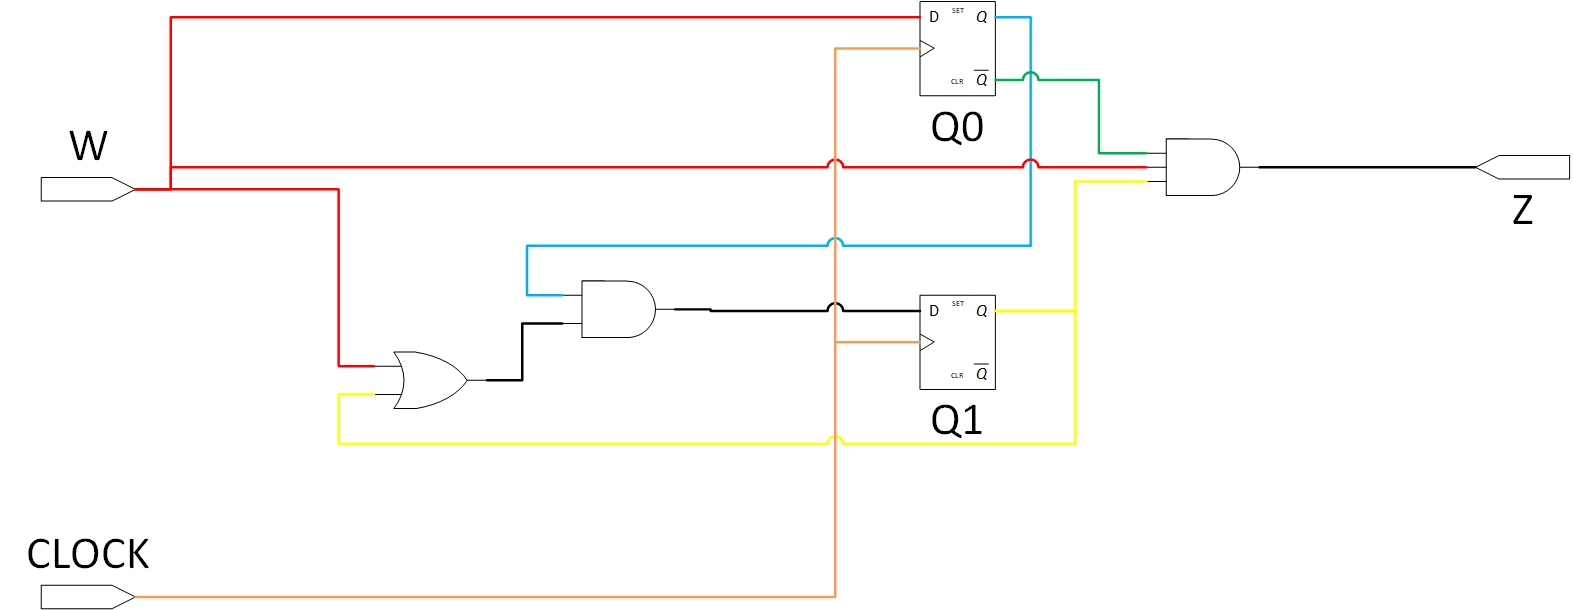
\includegraphics[width=14cm]{Imagenes/TP2_EJ2_MEALY_GREY.jpg}
\caption{Circuito lógico de Mealy }
\end{figure}

%% 	VERILOG MEALY

Con esto podemos concluir que el circuito de Mealy es mejor que el de Moore ya que utiliza menos integrados y realiza la misma función. Observando ambos circuitos pudimos ver que realizaban lo pedido de encontrar la secuencia.
\end{document}

\documentclass[10pt,a4paper]{article}
\usepackage{tikz}
\usetikzlibrary{matrix,calc}
\usepackage{multirow}
\usepackage[utf8]{inputenc}
\usepackage[spanish]{babel}
\usepackage{amsmath}
\usepackage{amsfonts}
\usepackage{amssymb}
\usepackage{graphicx}
\usepackage{float}
\usepackage[left=2cm,right=2cm,top=2cm,bottom=2cm]{geometry}
\usepackage{circuitikz}
\usepackage{tikz-timing}
\usetikztiminglibrary[rising arrows]{clockarrows}
\usepackage{pgfplots}
\pgfplotsset{compat=1.15}
\usepackage{listings}
\usepackage[export]{adjustbox}
\usepackage{graphicx,wrapfig,lipsum}
\usepackage{booktabs}
\usepackage[skip=0pt]{caption}
\captionsetup[figure]{font=small,labelfont=small}


\usetikzlibrary{matrix,calc}

%isolated term
%#1 - Optional. Space between node and grouping line. Default=0
%#2 - node
%#3 - filling color
\newcommand{\implicantsol}[3][0]{
    \draw[rounded corners=3pt, fill=#3, opacity=0.3] ($(#2.north west)+(135:#1)$) rectangle ($(#2.south east)+(-45:#1)$);
    }


%internal group
%#1 - Optional. Space between node and grouping line. Default=0
%#2 - top left node
%#3 - bottom right node
%#4 - filling color
\newcommand{\implicant}[4][0]{
    \draw[rounded corners=3pt, fill=#4, opacity=0.3] ($(#2.north west)+(135:#1)$) rectangle ($(#3.south east)+(-45:#1)$);
    }

%group lateral borders
%#1 - Optional. Space between node and grouping line. Default=0
%#2 - top left node
%#3 - bottom right node
%#4 - filling color
\newcommand{\implicantcostats}[4][0]{
    \draw[rounded corners=3pt, fill=#4, opacity=0.3] ($(rf.east |- #2.north)+(90:#1)$)-| ($(#2.east)+(0:#1)$) |- ($(rf.east |- #3.south)+(-90:#1)$);
    \draw[rounded corners=3pt, fill=#4, opacity=0.3] ($(cf.west |- #2.north)+(90:#1)$) -| ($(#3.west)+(180:#1)$) |- ($(cf.west |- #3.south)+(-90:#1)$);
}

%group top-bottom borders
%#1 - Optional. Space between node and grouping line. Default=0
%#2 - top left node
%#3 - bottom right node
%#4 - filling color
\newcommand{\implicantdaltbaix}[4][0]{
    \draw[rounded corners=3pt, fill=#4, opacity=0.3] ($(cf.south -| #2.west)+(180:#1)$) |- ($(#2.south)+(-90:#1)$) -| ($(cf.south -| #3.east)+(0:#1)$);
    \draw[rounded corners=3pt, fill=#4, opacity=0.3] ($(rf.north -| #2.west)+(180:#1)$) |- ($(#3.north)+(90:#1)$) -| ($(rf.north -| #3.east)+(0:#1)$);
}

%group corners
%#1 - Optional. Space between node and grouping line. Default=0
%#2 - filling color
\newcommand{\implicantcantons}[2][0]{
    \draw[rounded corners=3pt, opacity=.3] ($(rf.east |- 0.south)+(-90:#1)$) -| ($(0.east |- cf.south)+(0:#1)$);
    \draw[rounded corners=3pt, opacity=.3] ($(rf.east |- 8.north)+(90:#1)$) -| ($(8.east |- rf.north)+(0:#1)$);
    \draw[rounded corners=3pt, opacity=.3] ($(cf.west |- 2.south)+(-90:#1)$) -| ($(2.west |- cf.south)+(180:#1)$);
    \draw[rounded corners=3pt, opacity=.3] ($(cf.west |- 10.north)+(90:#1)$) -| ($(10.west |- rf.north)+(180:#1)$);
    \fill[rounded corners=3pt, fill=#2, opacity=.3] ($(rf.east |- 0.south)+(-90:#1)$) -|  ($(0.east |- cf.south)+(0:#1)$) [sharp corners] ($(rf.east |- 0.south)+(-90:#1)$) |-  ($(0.east |- cf.south)+(0:#1)$) ;
    \fill[rounded corners=3pt, fill=#2, opacity=.3] ($(rf.east |- 8.north)+(90:#1)$) -| ($(8.east |- rf.north)+(0:#1)$) [sharp corners] ($(rf.east |- 8.north)+(90:#1)$) |- ($(8.east |- rf.north)+(0:#1)$) ;
    \fill[rounded corners=3pt, fill=#2, opacity=.3] ($(cf.west |- 2.south)+(-90:#1)$) -| ($(2.west |- cf.south)+(180:#1)$) [sharp corners]($(cf.west |- 2.south)+(-90:#1)$) |- ($(2.west |- cf.south)+(180:#1)$) ;
    \fill[rounded corners=3pt, fill=#2, opacity=.3] ($(cf.west |- 10.north)+(90:#1)$) -| ($(10.west |- rf.north)+(180:#1)$) [sharp corners] ($(cf.west |- 10.north)+(90:#1)$) |- ($(10.west |- rf.north)+(180:#1)$) ;
}

%Empty Karnaugh map 4x4
\newenvironment{Karnaugh}%
{
\begin{tikzpicture}[baseline=(current bounding box.north),scale=0.8]
\draw (0,0) grid (4,4);
\draw (0,4) -- node [pos=0.7,above right,anchor=south west] {cd} node [pos=0.7,below left,anchor=north east] {ab} ++(135:1);
%
\matrix (mapa) [matrix of nodes,
        column sep={0.8cm,between origins},
        row sep={0.8cm,between origins},
        every node/.style={minimum size=0.3mm},
        anchor=8.center,
        ampersand replacement=\&] at (0.5,0.5)
{
                       \& |(c00)| 00         \& |(c01)| 01         \& |(c11)| 11         \& |(c10)| 10         \& |(cf)| \phantom{00} \\
|(r00)| 00             \& |(0)|  \phantom{0} \& |(1)|  \phantom{0} \& |(3)|  \phantom{0} \& |(2)|  \phantom{0} \&                     \\
|(r01)| 01             \& |(4)|  \phantom{0} \& |(5)|  \phantom{0} \& |(7)|  \phantom{0} \& |(6)|  \phantom{0} \&                     \\
|(r11)| 11             \& |(12)| \phantom{0} \& |(13)| \phantom{0} \& |(15)| \phantom{0} \& |(14)| \phantom{0} \&                     \\
|(r10)| 10             \& |(8)|  \phantom{0} \& |(9)|  \phantom{0} \& |(11)| \phantom{0} \& |(10)| \phantom{0} \&                     \\
|(rf) | \phantom{00}   \&                    \&                    \&                    \&                    \&                     \\
};
}%
{
\end{tikzpicture}
}

%Empty Karnaugh map 2x4
\newenvironment{Karnaughvuit}%
{
\begin{tikzpicture}[baseline=(current bounding box.north),scale=0.8]
\draw (0,0) grid (4,2);
\draw (0,2) -- node [pos=0.7,above right,anchor=south west] {bc} node [pos=0.7,below left,anchor=north east] {a} ++(135:1);
%
\matrix (mapa) [matrix of nodes,
        column sep={0.8cm,between origins},
        row sep={0.8cm,between origins},
        every node/.style={minimum size=0.3mm},
        anchor=4.center,
        ampersand replacement=\&] at (0.5,0.5)
{
                      \& |(c00)| 00         \& |(c01)| 01         \& |(c11)| 11         \& |(c10)| 10         \& |(cf)| \phantom{00} \\
|(r00)| 0             \& |(0)|  \phantom{0} \& |(1)|  \phantom{0} \& |(3)|  \phantom{0} \& |(2)|  \phantom{0} \&                     \\
|(r01)| 1             \& |(4)|  \phantom{0} \& |(5)|  \phantom{0} \& |(7)|  \phantom{0} \& |(6)|  \phantom{0} \&                     \\
|(rf) | \phantom{00}  \&                    \&                    \&                    \&                    \&                     \\
};
}%
{
\end{tikzpicture}
}

%Empty Karnaugh map 2x2
\newenvironment{Karnaughquatre}%
{
\begin{tikzpicture}[baseline=(current bounding box.north),scale=0.8]
\draw (0,0) grid (2,2);
\draw (0,2) -- node [pos=0.7,above right,anchor=south west] {b} node [pos=0.7,below left,anchor=north east] {a} ++(135:1);
%
\matrix (mapa) [matrix of nodes,
        column sep={0.8cm,between origins},
        row sep={0.8cm,between origins},
        every node/.style={minimum size=0.3mm},
        anchor=2.center,
        ampersand replacement=\&] at (0.5,0.5)
{
          \& |(c00)| 0          \& |(c01)| 1  \\
|(r00)| 0 \& |(0)|  \phantom{0} \& |(1)|  \phantom{0} \\
|(r01)| 1 \& |(2)|  \phantom{0} \& |(3)|  \phantom{0} \\
};
}%
{
\end{tikzpicture}
}

%Defines 8 or 16 values (0,1,X)
\newcommand{\contingut}[1]{%
\foreach \x [count=\xi from 0]  in {#1}
     \path (\xi) node {\x};
}

%Places 1 in listed positions
\newcommand{\minterms}[1]{%
    \foreach \x in {#1}
        \path (\x) node {1};
}

%Places 0 in listed positions
\newcommand{\maxterms}[1]{%
    \foreach \x in {#1}
        \path (\x) node {0};
}

%Places X in listed positions
\newcommand{\indeterminats}[1]{%
    \foreach \x in {#1}
        \path (\x) node {X};
}
\newenvironment{KarnaughTP3}%
{
\begin{tikzpicture}[baseline=(current bounding box.north),scale=0.8]
\draw (0,0) grid (4,4);
\draw (0,4) -- node [pos=0.9,above right,anchor=south west] {$Q_1 Q_0$} node [pos=0.7,below left,anchor=north east] {$W Q_2$} ++(135:1);
%
\matrix (mapa) [matrix of nodes,
        column sep={0.8cm,between origins},
        row sep={0.8cm,between origins},
        every node/.style={minimum size=0.3mm},
        anchor=8.center,
        ampersand replacement=\&] at (0.5,0.5)
{
                       \& |(c00)| 00         \& |(c01)| 01         \& |(c11)| 11         \& |(c10)| 10         \& |(cf)| \phantom{00} \\
|(r00)| 00             \& |(0)|  \phantom{0} \& |(1)|  \phantom{0} \& |(3)|  \phantom{0} \& |(2)|  \phantom{0} \&                     \\
|(r01)| 01             \& |(4)|  \phantom{0} \& |(5)|  \phantom{0} \& |(7)|  \phantom{0} \& |(6)|  \phantom{0} \&                     \\
|(r11)| 11             \& |(12)| \phantom{0} \& |(13)| \phantom{0} \& |(15)| \phantom{0} \& |(14)| \phantom{0} \&                     \\
|(r10)| 10             \& |(8)|  \phantom{0} \& |(9)|  \phantom{0} \& |(11)| \phantom{0} \& |(10)| \phantom{0} \&                     \\
|(rf) | \phantom{00}   \&                    \&                    \&                    \&                    \&                     \\
};
}%
{
\end{tikzpicture}
}

\newenvironment{KarnaughvuiteTP3}%
{
\begin{tikzpicture}[baseline=(current bounding box.north),scale=0.8]
\draw (0,0) grid (4,2);
\draw (0,2) -- node [pos=0.9,above right,anchor=south west] {$Q_1Q_0$} node [pos=0.7,below left,anchor=north east] {$W$} ++(135:1);
%
\matrix (mapa) [matrix of nodes,
        column sep={0.8cm,between origins},
        row sep={0.8cm,between origins},
        every node/.style={minimum size=0.3mm},
        anchor=4.center,
        ampersand replacement=\&] at (0.5,0.5)
{
                      \& |(c00)| 00         \& |(c01)| 01         \& |(c11)| 11         \& |(c10)| 10         \& |(cf)| \phantom{00} \\
|(r00)| 0             \& |(0)|  \phantom{0} \& |(1)|  \phantom{0} \& |(3)|  \phantom{0} \& |(2)|  \phantom{0} \&                     \\
|(r01)| 1             \& |(4)|  \phantom{0} \& |(5)|  \phantom{0} \& |(7)|  \phantom{0} \& |(6)|  \phantom{0} \&                     \\
|(rf) | \phantom{00}  \&                    \&                    \&                    \&                    \&                     \\
};
}%
{
\end{tikzpicture}
}
\newenvironment{KarnaughquatreTP3}%
{
\begin{tikzpicture}[baseline=(current bounding box.north),scale=0.8]
\draw (0,0) grid (2,2);
\draw (0,2) -- node [pos=0.7,above right,anchor=south west] {$Q_0$} node [pos=0.7,below left,anchor=north east] {$Q_1$} ++(135:1);
%
\matrix (mapa) [matrix of nodes,
        column sep={0.8cm,between origins},
        row sep={0.8cm,between origins},
        every node/.style={minimum size=0.3mm},
        anchor=2.center,
        ampersand replacement=\&] at (0.5,0.5)
{
          \& |(c00)| 0          \& |(c01)| 1  \\
|(r00)| 0 \& |(0)|  \phantom{0} \& |(1)|  \phantom{0} \\
|(r01)| 1 \& |(2)|  \phantom{0} \& |(3)|  \phantom{0} \\
};
}%
{
\end{tikzpicture}
}


\begin{document}
\section{Ejercicio 3}
\subsection{Moore}
Se nos dio un diagrama de estado y se nos pidió implementar una máquina de estado de Moore que la resolviera. Para esto hicimos un análisis con tablas que muestre las transiciones de estados, y luego vimos como serían las transiciones con Flip Flop D (). Como ya hicimos anteriormente utilizamos mapas de Karnaugh para resolver el problema. 

%%	DIAGRAMA

\begin{figure}[hbtp]
	\centering
	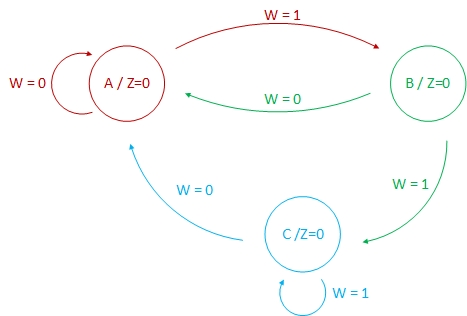
\includegraphics[width=8cm]{Imagenes/mooreej3.jpg}
	\caption{Diagrama Moore }
\end{figure}


%%	TABLA DE TRANSICIONES

\begin{figure}[hbtp]
	\begin{center}
		\begin{tabular}{|c|c|c|c|}
\hline
\multirow{2}{*}{\textbf{ESTADO ACTUAL}} & \multicolumn{2}{c|}{\textbf{ESTADO SIGUIENTE}} & \textbf{SALIDA} \\ \cline{2-4} 
 & \textbf{W=0} & \textbf{W=1} & \textbf{Z} \\ \hline
\textbf{A} & \textbf{A} & \textbf{B} & \textbf{0} \\ \hline
\textbf{B} & \textbf{A} & \textbf{C} & \textbf{1} \\ \hline
\textbf{C} & \textbf{A} & \textbf{C} & \textbf{0} \\ \hline
\textbf{D} & \textbf{X} & \textbf{X} & \textbf{X} \\ \hline
		\end{tabular}
		\caption{Transiciones de Estados - Máquina de Moore} 
		\label{3_fig1}
	\end{center}
\end{figure}


%	TRANSICIONES CON FLIP FLOP
\begin{figure}[hbtp]
	\begin{center}
		\begin{tabular}{|c|c|c|c|c|c|c|}
\hline
\multicolumn{2}{|c|}{\multirow{2}{*}{\textbf{ESTADO ACTUAL}}} & \multicolumn{4}{c|}{\textbf{ESTADO SIGUIENTE}} & \multirow{2}{*}{\textbf{SALIDA}} \\ \cline{3-6}
\multicolumn{2}{|c|}{} & \multicolumn{2}{c|}{\textbf{W = 0}} & \multicolumn{2}{c|}{\textbf{W = 1}} &  \\ \hline
\textbf{$Q_{1_{t}}$} & \textbf{$Q_{0_{t}}$} & \textbf{$Q_{1_{t+1}}$} & \textbf{$Q_{0_{t+1}}$} & \textbf{$Q_{1_{t+1}}$} & \textbf{$Q_{0_{t}}$} & \textbf{Z} \\ \hline
\textbf{0} & \textbf{0} & \textbf{0} & \textbf{0} & \textbf{0} & \textbf{1} & \textbf{0} \\ \hline
\textbf{0} & \textbf{1} & \textbf{0} & \textbf{0} & \textbf{1} & \textbf{0} & \textbf{1} \\ \hline
\textbf{1} & \textbf{0} & \textbf{0} & \textbf{0} & \textbf{1} & \textbf{0} & \textbf{0} \\ \hline
\textbf{1} & \textbf{1} & \textbf{X} & \textbf{X} & \textbf{X} & \textbf{X} & \textbf{X} \\ \hline
		\end{tabular}
		\caption{Transiciones con Flip Flop - Máquina de Moore} 
		\label{3_fig2}
	\end{center}
\end{figure}


%	MAPA Karnaugh Q0
\begin{figure}[H]
	\begin{center}
		\begin{KarnaughvuiteTP3}
		\minterms{4}
		\maxterms{0,1,2,5,6}
		\indeterminats{3,7}
		\implicant{4}{4}{orange}
		\end{KarnaughvuiteTP3}
	\end{center}
	\caption{$Q_0$: Máq. de Moore} 
	\label{3_fig3}
\end{figure}

%	MAPA Karnaugh Q1
\begin{figure}[H]
	\begin{center}
		\begin{KarnaughvuiteTP3}
		\minterms{5,6}
		\maxterms{0,1,2,4}
		\indeterminats{3,7}
		\implicant{5}{7}{orange}
		\implicant{7}{6}{blue}
		\end{KarnaughvuiteTP3}
	\end{center}
	\caption{$Q_1$ Máq. de Moore} 
	\label{3_fig4}
\end{figure}

%	MAPA Karnaugh Z
\begin{figure}[H]
	\begin{center}
		\begin{KarnaughquatreTP3}
		\minterms{1}
		\maxterms{0,2}
		\indeterminats{3}
		\implicantsol{1}{green}
		\end{KarnaughquatreTP3}
	\end{center}
	\caption{$Z$: Máq. de Moore} 
	\label{3_fig5}
\end{figure}



%% EXPLICACION DEL ANALISIS
Al reducir los minitérminos obtuvimos las siguientes expresiones que representan el circuito lógico que se usara para resolver la máquina de estado:

\begin{align*}
	Q_{0_{t+1}} &= W * \overline{Q_{1}} * \overline{Q_{0}}\\
	Q_{1_{t+1}} &= W * (Q_{1} + Q_{0})  \\
	Z &= Q_{0} \\
\end{align*}


Entonces el circuito quedará de la siguiente manera:

\begin{figure}[H]
	\centering
	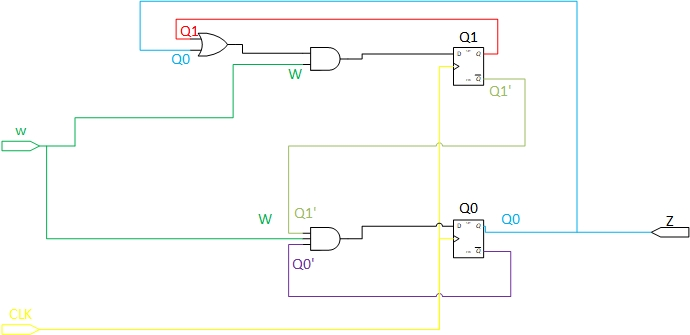
\includegraphics[width=8cm]{Imagenes/circej3moore.jpg}
	\caption{Circuito lógico - Moore}
	\label{3_fig6}
\end{figure}


\subsection{Mealy}
Analizando las tablas de transiciones de estados pudimos notar que la función de la máquina es prender la salida cuando se recibe la primer señal en HIGH y luego se apaga en el segundo CLOCK. Para implementar ahora la máquina de Mealy tuvimos en cuenta esto y diseñamos el siguiente diagrama.

%% DIAGRAMA DE MEALY
\begin{figure}[hbtp]
	\centering
	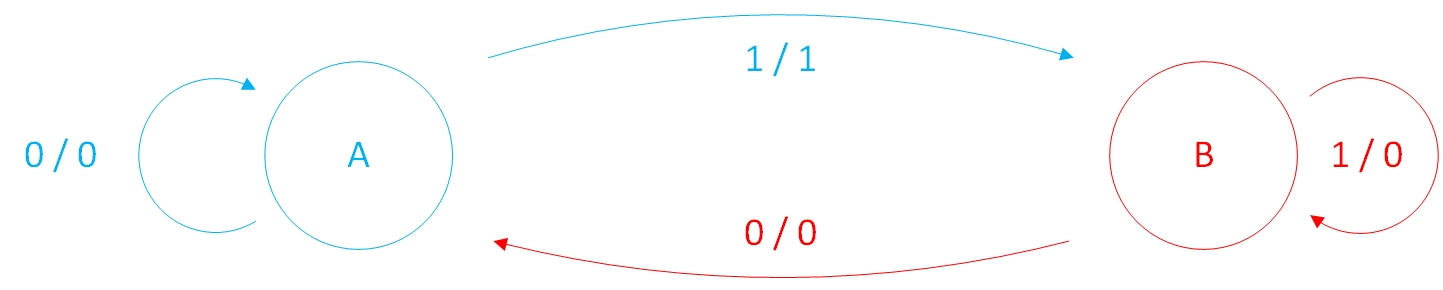
\includegraphics[width=8cm]{Imagenes/mealyej3.jpg}
	\caption{Diagrama de Mealy}
\end{figure}

De este diagrama representamos en una tabla la transiciones de estados directamente con un Flip Flop, ya que al haber solo 2 estados solo se necesita un Flip Flop para representar ambos estados, el estado 0 y estado 1. La tabla es la siguiente:

\begin{figure}[H]
	\begin{center}
		\begin{tabular}{|c|c|c|c|c|}
\hline
\multirow{2}{*}{\textbf{ESTADO ACTUAL}} & \multicolumn{2}{c|}{\textbf{ESTADO SIGUIENTE}} & \multicolumn{2}{c|}{\textbf{SALIDA}} \\ \cline{2-5} 
 & \multicolumn{2}{c|}{\textbf{Q}} & \multicolumn{2}{c|}{\textbf{Z}} \\ \hline
\textbf{Q} & \textbf{W=0} & \textbf{W=1} & \textbf{W=0} & \textbf{W=1} \\ \hline
\textbf{0} & \textbf{0} & \textbf{1} & \textbf{0} & \textbf{1} \\ \hline
\textbf{1} & \textbf{0} & \textbf{1} & \textbf{0} & \textbf{0} \\ \hline
		\end{tabular}
		\caption{Transiciones con Flip Flop - Máquina de Moore} 
		\label{3_fig8}
	\end{center}
\end{figure}

Sin un análisis muy complejo, el flip flop devuelve una salida en HIGH solo cuando la entrada es HIGH, e igualmente cuando devuelven una señal LOW, por lo que la salida será directamente la entrada. Pero la salida depende tanto del estado como de la entrada, característica de este tipo de máquina de estado, por lo que la salida será:

\begin{align*}
	Z &= W * \overline{Q_{0}} \\
\end{align*}
El circuito lógico queda muy simple a comparación del logrado con Moore, demostrado en la siguiente figura:

\begin{figure}[H]
	\centering
	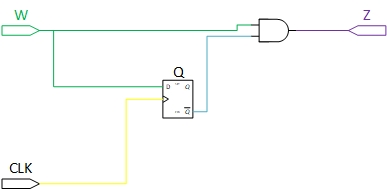
\includegraphics[width=8cm]{Imagenes/circej3mealy.jpg}
	\caption{Circuito lógico Mealy}
\end{figure}


\subsection{Implementación}
Para crear ambas máquinas se pidió que las entradas y salidas del circuito deberán ser lógica de 5V, mientras que toda la lógica interna trabajará con 3,3V. Para esto hicimos un circuito que pueda bajar de 5V a 3,3V y viceversa.

\begin{figure}[H]
	\centering
	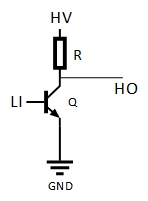
\includegraphics[scale=1]{Imagenes/Conversor.jpg}
	\caption{Conversor}
\end{figure}

Observamos que las tecnologías TTL y CMOS aceptaban bien los valores de 3,3V como señal HIGH para estos circuitos, por lo que no tuvimos restricción con respecto a las tecnologías.
En la siguiente imagen se puede ver como la salida cambia cuando el clock es HIGH y la entrada también, pero al segundo CLOCK se apaga aunque la entrada siga en HIGH, demostrando que solo se prende con el primer 1 lógico recibido.
\begin{figure}[H]
	\centering
	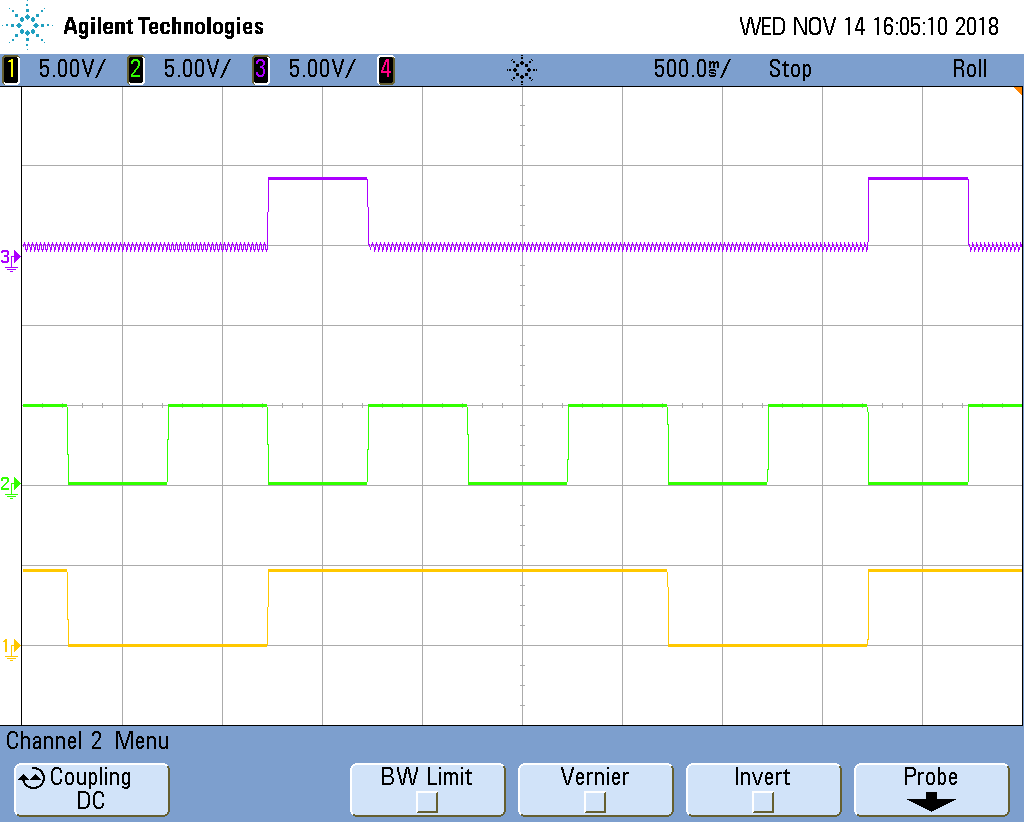
\includegraphics[width=14cm]{Imagenes/MedicionTP3_Ej3.png}
	\caption{Medición del Ejercicio 3}
\end{figure}

\subsection{Conclusión}
Pudimos observar el buen funcionamiento de ambas máquinas cumpliendo la misma función, aunque el circuito resuelto con Mealy necesito solo 2 componentes (que serían 2 integrados) por lo que resulta más simple y económico, también tiene menos delay la salida ya que solo consta de una compuerta.


\end{document}
\end{document}